\newcommand{\decktitle}{Python II - Grundlagen}

%%%%%%%%%%%%%%%%%%%%%%%%%%%%%%%%%%%%%%%%%%%%%%%%%
%
% DOCUMENT
%
%%%%%%%%%%%%%%%%%%%%%%%%%%%%%%%%%%%%%%%%%%%%%%%%%

\begin{frame}
    \subtitle{\decktitle}
    \titlepage
\end{frame}


\begin{frame}
    \frametitle{\textbf{Outline:}}
    \tableofcontents
\end{frame}

		
        
    \section{Variablen}
    
        \begin{frame}[fragile]{Variablen - Deklaration}
            In Python ist kein spezieller Befehl nötig, um Variablen zu erzeugen und zu deklarieren. Es muss lediglich festgelegt werden, wie der Name der Variable lautet und welcher Wert ihr zugewiesen wird. \\~\

\begin{pyconcode}
>>> x = 1
>>> y = 3.14
>>> z = "Hello world"
\end{pyconcode}
    
            In obigen Beispiel wurden 3 Variablen mit den Namen $x$, $y$ und $z$ erzeugt und ihnen jeweils die Werte $1$, $3.14$ und \code{"Hello world"} zugewiesen.
            
        \end{frame}
        
        \begin{frame}[fragile]{Mehrfachzuweisung}
            Auf der linken Seite der Variablenzuweisung steht immer der Variablenname, dann folgt ein \code{=}-Zeichen und auf der rechten Seite wird der Wert festgelegt. \\~\
            
            In Python folgt nach jeder Anweisung eine neue Zeile, Folgendes ist also nicht erlaubt: 
\begin{pyconcode}
>>> x = 1, y = 3.14
\end{pyconcode}

            Es können jedoch trotzdem mehrere Variablen innerhalb einer Zeile deklariert werden \textit{(Multiple Assignment)}:
\begin{pyconcode}
>>> x, y = 1, 3.14
\end{pyconcode}
            
            Auf diese Weise wird ebenso wie oben der Variable \code{x} der Wert \code{1} und der Variable \code{y} der Wert \code{3.14} zugewiesen
            
        \end{frame}
        
        \begin{frame}[fragile]{Wertüberschreibung}
        
            Nachdem einer Variablen ein Wert zugewiesen wurde, kann diese im Anschluss ohne Umstände auch mit einem anderen Wert überschrieben werden:
  
\begin{pyconcode}
>>> x = 1
>>> x = 5
>>> x
5
\end{pyconcode}
            Der Variablen \code{x} wurde zunächst der Wert \code{1} zugewiesen und anschließend mit dem Wert \code{5} überschrieben. \code{x} besitzt nun also den Wert \code{5}. 
            Eine Variable kann auch mit einem Wert eines anderen Datentyps überschrieben werden:

\begin{pyconcode}
>>> x = 1
>>> x = "Hello world"
>>> x
"Hello world"
\end{pyconcode}

        \end{frame}
        
        \begin{frame}[fragile]{Ausgabe}
            Um sich den aktuellen Wert einer Variablen anzeigen zu lassen, muss im interaktiven Modus des Python-Interpreters lediglich der Name der Variable eingegeben werden, der Wert wird dann als Ausgabe in der nächsten Zeile angezeigt:
\begin{pyconcode}
>>> x = 1
>>> x
1
\end{pyconcode}

            Alternativ kann auch die \code{print()}-Funktion genutzt werden, um Werte auszugeben:
\begin{pyconcode}
>>> x = 1
>>> print(x)
1
\end{pyconcode}

        \end{frame}
        
        \begin{frame}[fragile]{Ausgabe}
            \begin{alertblock}{Achtung}
                Die 1. Methode, bei der lediglich der Variablenname "ausgeführt" wird, funktioniert nur im interaktiven Modus des Interpreters. Wird der Code innerhalb einer Datei o.ä. ausgeführt, muss immer die \code{print()}-Funktion genutzt werden.
            \end{alertblock}
        
        \end{frame}
        
        \begin{frame}{Benamungsregeln \& -konventionen}
            \textbf{Regeln}: Variablennamen
            \begin{itemize}
                \item \textbf{müssen} mit einem Buchstaben oder einem Underscore (\_) beginnen
                \item \textbf{dürfen nicht} mit einer Zahl/Ziffer beginnen
                \item \textbf{dürfen lediglich} aus alphanumerischen Zeichen (A-Z, a-z, 0-9) und Underscores (\_) bestehen
                \item sind case-sensitive (Groß-/ Kleinschreibung wird unterschieden, z.B. $x \neq X$)
            \end{itemize}
            
            \textbf{Konventionen}: Variablennamen
            \begin{itemize}
                \item \textbf{sollten} möglichst aussagekräftig sein (z.B. ist der Variablenname \code{x} kaum aussagekräftig, \code{age} dagegen schon)
                \item bestehen i.d.R. nur aus Kleinbuchstaben, wobei einzelne Wörter durch Underscores getrennt werden (z.B. \code{age\_of\_person}), wird als \textit{Snake case (snake\_case)} bezeichnet\footnote{In manchen anderen Programmiersprachen (z.B. Java) wird überwiegend \textit{Camel case (camelCase)} genutzt, wobei Wörter nicht durch Underscores getrennt werden, sondern der erste Buchstabe eines Wortes groß geschrieben wird (z.B. \texttt{ageOfPerson})}
            \end{itemize}
        \end{frame}
        
        \begin{subsection}{Aufgaben}
            
            \begin{frame}{Aufgaben}
            
                \begin{enumerate}
                    \item Wie werden in Python Variablen erzeugt?
                    \item Wie können den Variablen \code{name} und \code{age} innerhalb einer Zeile verschiedene Werte zugewiesen werden?
                    \item Sind Variablenwerte konstant? Wie können sie verändert werden?
                    \item Welche der folgenden Variablennamen sind valide?
                        \begin{itemize}
                            \item \texttt{\_name}
                            \item \texttt{name\_}
                            \item \texttt{Name}
                            \item \texttt{int}
                            \item \texttt{int\$}
                            \item \texttt{name\_and\_age}
                            \item \texttt{nameAndAge}
                            \item \texttt{name and age}
                            \item \texttt{1variable}
                            \item \texttt{variable1}
                        \end{itemize}
                    \item Was muss bei der Ausgabe von Werten im interaktiven Interpreter bzw. der Ausführung des Codes in Dateien beachtet werden?
                    \item Wie sollten Variablen in Python benamt werden?
                \end{enumerate}
                
            \end{frame}
        \end{subsection}
        
    \section{Kommentare}
        \begin{frame}{Kommentare (I)}
            Wie in den meisten anderen Programmiersprachen besteht in Python die Möglichkeiten, den Code mit Kommentaren anzureichern. \\~\
            
            Kommentare dienen dazu, Informationen im Code zu ergänzen, um beispielsweise die Funktionalität zu beschreiben bzw. dokumentieren, anderen Entwicklern eine Hilfestellung zu geben, den Code besser verstehen zu können oder auch komplexe Sachverhalte in natürlicher Sprache wiederzugeben, die in Codeform nur schwer verständlich sind. \\~\

            Kommentare werden vom Interpreter nicht berücksichtigt, daher können Kommentare einen beliebigen Inhalt besitzen.
        \end{frame}
        
        \begin{frame}[fragile]{Kommentare (II) - Einzeilige Kommentare}
            
            Kurze Kommentare werden mit einem \code{\#}-Zeichen vorangestellt. Diese Kommentare gelten nur bis zum jeweiligen Zeilenende.

\begin{pythoncode}
# Das ist ein Kommentar.            
x = 1 #  Das ist ein Kommentar, der erst nach der Variablenzuweisung beginnt
\end{pythoncode}
        \end{frame}
        
        \begin{frame}[fragile]{Kommentare (III) - Mehrzeilige Kommentare}
            
            Manchmal (insbesondere bei der Beschreibung komplexer Sachverhalte) können sich Kommentare auch über viele Zeilen erstrecken. Um nicht explizit jede Zeile mit \code{\#} voranstellen zu müssen, gibt es in Python die Möglichkeit, mehrzeilige Kommentare zu erzeugen.
            
            Mehrzeilige Kommentare werden mit 3 Anführungszeichen (\code{"""}) eingeleitet und auch wieder beendet.
            Alles was dazwischen enthalten ist wird als Kommentar behandelt und vom Interpreter ignoriert.
\begin{pythoncode}
"""
Das ist ein mehrzeiliger Kommentar.

Alles was zwischen den Anführungszeichen steht wird vom Interpreter ignoriert.
Hier ist der Kommentar beendet
"""
\end{pythoncode}
        \end{frame}
    
    \section{Datentypen}
    
        \begin{frame}{Datentypen}
            Da Python eine typisierte Sprache ist, besitzt jede Variable auch einen Datentypen. Datentypen beschreiben, welche Art von Wert in einer Variablen gespeichert ist. \\~\
            
            \begin{block}{Hinweis}
                Um zu überprüfen, welchen Datentypen eine Variable besitzt, gibt es in Python die \code{type()}-Funktion. Um bspw. den Datentypen der Variablen \code{x} festzustellen, kann die Funktion folgendermaßen aufgerufen werden: \code{type(x)}
            \end{block}
        \end{frame}
        
        \begin{frame}[fragile]{Numerische Datentypen (I)}
            
            Numerische Datentypen beschreiben Zahlenwerte unterschiedlicher Art:
            
            \begin{itemize}
                \item \textbf{integer}: Positive und negative Ganzzahlen (keine Nachkommastellen). \\~\
                Bezeichnung in Python: \textbf{\code{int}}
\begin{pyconcode}
>>> x = 5
>>> type(x)
<class 'int'>
\end{pyconcode}
            
                \item \textbf{float}: Positive und negative reelle Zahlen mit Fließkommadarstellung (mit Nachkommastellen). \\~\
                Bezeichnung in Python: \textbf{\code{float}}
\begin{pyconcode}
>>> x = 3.14
>>> type(x)
<class 'float'>
\end{pyconcode}

            \end{itemize}
        \end{frame}
        
        
        \begin{frame}[fragile]{Numerische Datentypen (II)}
        
            \begin{itemize}
                \item \textbf{complex}:Komplexe Zahlen mit einem reellen und einem imaginären Anteil. Sowohl der reelle als auch der komplexe Anteil wird durch \code{float}-Zahlen dargestellt. In der Ausgabe wird der imaginäre Teil durch ein \code{j} gekennzeichnet, um deutlich zu machen, dass es sich dabei um eine imaginäre Zahl handelt. Im Beispiel unten wird eine komplexe Zahl mit dem reellen Anteil \code{1} und dem imaginären Anteil \code{0} erzeugt. \\~\
                Bezeichnung in Python: \textbf{\code{complex}}
\begin{pyconcode}
>>> x = complex(1,0)
>>> x
(1+0j)
>>> type(x)
<class 'complex'>
\end{pyconcode}
            \end{itemize}
            
        \end{frame}
        
         \begin{frame}[fragile]{Numerische Datentypen (III)}
            \begin{alertblock}{Achtung}
                Bei der Verwendung von Kommazahlen muss auf die korrekte Verwendung des Dezimaltrennzeichens geachtet werden. Da die Schreibweisen in der Informatik meist auf dem englischen System basieren, wird als Dezimaltrennzeichen ein Punkt und kein Komma verwendet (z.B. \code{3.14} anstatt \code{3,14}).
            \end{alertblock}
         \end{frame}
        
        
        \begin{frame}[fragile]{Boolesche Datentypen}
        
            \begin{itemize}
                \item \textbf{boolean}: Benannt nach George Boole. Stellt einen einfachen Zustandswert dar. Es gibt lediglich zwei Zustände: Wahr und Falsch (analog: Binärdarstellung (1 / 0), Schalterdarstellung (An / Aus)). \\~\
                Bezeichnung in Python: \textbf{\code{bool}}
\begin{pyconcode}
>>> x = True
>>> y = False
>>> type(x)
<class 'bool'>
>>> type(y)
<class 'bool'>
\end{pyconcode}

            \begin{alertblock}{Achtung}
                \code{True} und \code{False} sind eingebaute Schlüsselwörter in Python und daher case-sensitive. \code{true} bzw. \code{false} sind keine validen booleschen Werte.
            \end{alertblock}
            
            \end{itemize}
            
        \end{frame}
        
        \begin{frame}[fragile]{Zeichenketten (I)}
        
            \begin{itemize}
                \item \textbf{string}: Zeichenketten, meist \textit{strings} genannt, sind eine Folge von einzelnen Zeichen, Buchstaben und Ziffern, die als Buchstaben behandelt werden, die von einfachen (\code{'}) oder doppelten (\code{"}) Anführungszeichen eingeschlossen werden.\\~\
                Bezeichnung in Python: \textbf{\code{str}}
\begin{pyconcode}
>>> x = 'Hello world'
>>> type(x)
<class 'str'>
>>> y = "1234"
>>> type(y)
<class 'str'>
\end{pyconcode}

            \begin{alertblock}{Achtung}
                Ein String wird entweder von einfachen oder doppelten Anführungszeichen eingeschlossen, eine Kombination innerhalb eines Strings ist aber \textbf{nicht} erlaubt (z.B. \code{"Hello world'})
            \end{alertblock}
            
            \end{itemize}
            
        \end{frame}
        
        \begin{frame}[fragile]{Zeichenketten (II)}
            Zeichenketten müssen nicht zwangsläufig statisch angelegt werden, sondern können auch dynamisch erzeugt werden, d.h. mit den Werten anderer Variablen ergänzt werden.\\~\
            
            
            Hierfür können sogenannte \textbf{f-Strings} verwendet werden. Um diese zu nutzen, muss die Zeichenkette mit einem "f" ("formatiert") vorangestellt werden. Variablenwerte, die in den String eingefügt werden sollen, werden innerhalb des Strings mit geschweiften Klammern (\code{\{\}}) injiziert.
\begin{pythoncode}
>>> first_name = 'John'
>>> age = 42

>>> print(f"Hallo {first_name}, du bist {age} Jahre alt")
"Hallo John, du bist 42 Jahre alt"
        
\end{pythoncode}
        
        \end{frame}
        
        \begin{frame}[fragile]{Zeichenketten (III)}
        Alternativ können Zeichenketten auch mit einen \code{+}-Zeichen konkateniert (zusammengesetzt) werden.
        
        \begin{alertblock}{Achtung}
                String-Konkatenation mithilfe des Addition-Operators funktioniert nur zwischen Strings, andere Datentypen müssen vor der Konkatenation zunächst in den String-Datentyp konvertiert werden.
            \end{alertblock}
\begin{pythoncode}
>>> first_name = 'John'
>>> age = 42

>>> print("Hallo " + first_name + ", du bist " + age +  " Jahre alt")
TypeError: can only concatenate str (not "int") to str

>>> print("Hallo " + first_name + ", du bist " + str(age) +  " Jahre alt")
"Hallo John, du bist 42 Jahre alt"
        \end{pythoncode}       
            
        
        \end{frame}
        
        \begin{frame}[fragile, allowframebreaks]{Zeichenketten (IV)}
            Zur Zeichenkettenverarbeitung stehen weitere Funktionen zur Verfügung, die bereits standardmäßig in Python enthalten sind sind.
            
            \begin{itemize}
                \item \code{upper()}: Wandelt String in Großbuchstaben um (analog dazu: \code{lower()})
\begin{pythoncode}
>>> "Hello".upper()
"HELLO"
\end{pythoncode}
                \item \code{startswith()}: Überprüft, ob ein String mit einer bestimmten Zeichenkette beginnt und liefert dementsprechend einen booleschen Wert zurück (analog dazu: \code{endswith()})
\begin{pythoncode}
>>> "Hello John".startswith("Hello")
True
\end{pythoncode}

                \item \code{split()}: Trennt einen String anhand der gewünschten Zeichen und gibt die Bestandteile als Liste zurück. Falls kein Parameter angegeben wird, wird standardmäßig anhand von Leerzeichen getrennt
\begin{pythoncode}
>>> "Hello John".split()
["Hello", "John"]

>>> "This.sentence.is.dot.separated".split(".")
['This', 'sentence', 'is', 'dot', 'separated']
\end{pythoncode}
            \end{itemize}
            
In Python stehen viele weitere String-Funktionen zur Verfügung. Eine vollständige Beschreibung dieser Funktionen kann in der \href{https://docs.python.org/3/library/stdtypes.html#string-methods}{offiziellen Dokumentation} eingesehen werden.
        \end{frame}
        
        \begin{frame}[fragile]{None}
            
            Um zu kennzeichnen, dass eine Variable existiert, diese jedoch keinen Wert beinhaltet, also \textit{leer} ist, gibt es den Datentyp und das Schlüsselwort \code{None}.\\~\
            
            \begin{alertblock}{Achtung}
                \code{None} besitzt eine andere semantische und logische Bedeutung als der Wert \code{0}. \code{0} bedeutet, dass ein Wert vorhanden ist, dieser aber \texttt{0} beträgt, also einen numerischen Wert trägt. \code{None} dagegen bedeutet, dass überhaupt kein Wert gesetzt ist, daher handelt es sich auch nicht um einen numerischen Datentyp.
            \end{alertblock}

\begin{pyconcode}
>>> x = None
>>> type(x)
<class 'NoneType'>
>>> print(x)
None
>>> x is None
True
>>> x == None
True
>>> x == 0
False
\end{pyconcode}            
            
         \end{frame}
        
         \begin{frame}[fragile]{Weitere Datentypen}
            
            \begin{itemize}
                \item \textbf{Sequence} Datentypen: Sammlung mehrerer Werte (gleicher oder unterschiedlicher Datentypen) innerhalb einer Variable, z.B. \code{list}, \code{tuple}, \code{range}
                
                \item \textbf{Mapping} Datentypen: Sammlung mehrerer Werte (gleicher oder unterschiedlicher Datentypen) nach dem Key-Value Prinzip, z.B. \code{dict} (Dictionary/Wörterbuch)
                
                \item \textbf{Set} Datentypen: Sammlung mehrerer Werte (gleicher oder unterschiedlicher Datentypen) ohne Duplikate innerhalb einer Variable, z.B. \code{set}
                
                \item \textbf{Binäre} Datentypen: Darstellung von Zahlen im Binärsystem, z.B. \code{bytes}.
            \end{itemize}\\~\
            
            Sequence, Mapping und Set Datentypen werden im Abschnitt \nameref{subs:datastruct} näher erläutert, binäre Datentypen werden in diesem Rahmen nicht besprochen.
         \end{frame}
         
         
        \begin{frame}[fragile]{Konvertierungen (I)}
            Da Python schwach typisiert ist, können Variablen prinzipiell ohne weiteres in andere Datentypen umgewandelt werden. Hierfür stehen bereits standardmäßig Funktionen zu Verfügung, die genutzt werden können:
            
            \begin{table}[]
                \begin{tabular}{|l|c|c|c|c|c|}
                    \hline
                    \rowcolor[HTML]{EFEFEF} 
                    Umwandlung in ...                & Integer & Float   & Complex   & Boolescher Wert & String \\ \hline
                    \cellcolor[HTML]{EFEFEF}Funktion & int()   & float() & complex() & bool()          & str()  \\ \hline
                \end{tabular}
            \end{table}
            
\begin{pyconcode}
>>> x = 5
>>> type(x)
<class 'int'>
>>> y = float(x)
>>> type(y)
<class 'float'>
>>> y
5.0
\end{pyconcode}
        \end{frame}
    
        \begin{frame}[fragile]{Konvertierungen (II)}
            
            Bei Typkonvertierungen muss immer darauf geachtet werden, ob die Konvertierung \colorbox{good}{problemlos möglich} ist, u.U. mit \colorbox{medium}{Datenverlust oder Fehlern} gerechnet werden muss oder grundsätzlich \colorbox{bad}{nicht möglich} ist.
   
           \begin{table}[]
                \centering
                \resizebox{\textwidth}{!}{%
                \begin{tabular}{|l|c|c|c|c|c|}
                    \hline
                    \cellcolor[HTML]{EFEFEF} \diagbox{Von...}{zu...}
                    &
                    \multicolumn{1}{l|}{\cellcolor[HTML]{EFEFEF}int}
                    & 
                    \multicolumn{1}{l|}{\cellcolor[HTML]{EFEFEF}float}
                    & 
                    \multicolumn{1}{l|}{\cellcolor[HTML]{EFEFEF}complex}                     & 
                    \multicolumn{1}{l|}{\cellcolor[HTML]{EFEFEF}bool}                        & 
                    \multicolumn{1}{l|}{\cellcolor[HTML]{EFEFEF}str}                         \\ \hline


%% int row
\cellcolor[HTML]{EFEFEF}int     &                                                           

\cellcolor[HTML]{9AFF99} & 

\cellcolor[HTML]{9AFF99} \begin{tabular}[c]{@{}c@{}}Zahl besitzt zusätzlich\\ Dezimalstelle\\ \\ \code{float(5)} \Rightarrow \code{5.0}\end{tabular} & 

\cellcolor[HTML]{9AFF99} \begin{tabular}[c]{@{}c@{}}Integerzahl als reelle Zahl,\\ kein imaginärer Anteil\\ \\ \code{complex(5)} \Rightarrow \code{(5+0j)}\end{tabular} &

\cellcolor[HTML]{9AFF99} \begin{tabular}[c]{@{}c@{}}0 wird zu \code{False} ausgewertet,\\ alle anderen Zahlen zu \code{True}\\ \\ \code{bool(5)} \Rightarrow \code{True}\\ \code{bool(0)} \Rightarrow \code{False}\end{tabular} & 

\cellcolor[HTML]{9AFF99} \begin{tabular}[c]{@{}c@{}}String mit der Zahl als Inhalt\\ \\ \code{str(5)} \Rightarrow \code{'5'}\end{tabular}                                           

\\ \hline

% float row
\cellcolor[HTML]{EFEFEF}float   & 

\cellcolor[HTML]{FFFE65}\begin{tabular}[c]{@{}c@{}}Datenverlust, falls Zahl einen \\ Nachkommawert $\neq 0$ hat \\ (Nachkommastellen werden abgeschnitten) \\ \\ \code{int(5.0)} \Rightarrow \code{5}\\ \code{int(5.9)} \Rightarrow \code{5}\end{tabular} &                  

\cellcolor[HTML]{9AFF99} & 

\cellcolor[HTML]{9AFF99} \begin{tabular}[c]{@{}c@{}}Floatzahl als reelle Zahl,\\ kein imaginärer Anteil\\ \\ \code{complex(5.0)} \Rightarrow \code{5.0+0j}\end{tabular} & 

\cellcolor[HTML]{9AFF99} \begin{tabular}[c]{@{}c@{}}0.0 wird zu \code{False} ausgewertet,\\ alle anderen Zahlen zu \code{True}\\ \\ \code{bool(5.0)} \Rightarrow \code{True}\\ \code{bool(0.0)} \Rightarrow \code{False}\end{tabular} & 

\cellcolor[HTML]{9AFF99} \begin{tabular}[c]{@{}c@{}}String mit der Zahl als Inhalt\\ \\ \code{str(5.0)} \Rightarrow \code{'5.0'}\end{tabular}                                                             
\\ \hline

% complex row
\cellcolor[HTML]{EFEFEF}complex & 

\cellcolor[HTML]{FD6864}nicht möglich &

\cellcolor[HTML]{FD6864}nicht möglich &

\cellcolor[HTML]{9AFF99} & 

\cellcolor[HTML]{9AFF99} \begin{tabular}[c]{@{}c@{}}Wenn sowohl der reelle als auch der imaginäre Teil 0 ist,\\ wird der Ausdruck zu \code{True} ausgewertet,\\ ansonsten zu \code{False}\\ \\ \code{bool(complex(5,0))} \Rightarrow \code{True}\\ \code{bool(complex(0,0))} \Rightarrow \code{False}\end{tabular} &

\cellcolor[HTML]{9AFF99}\begin{tabular}[c]{@{}c@{}}String mit der komplexen Zahl als Inhalt\\ \\ \code{str(complex(5,2))} \Rightarrow \code{'(5+2j)'}\end{tabular}                                       

\\ \hline

% bool row

\cellcolor[HTML]{EFEFEF}bool    & 

\cellcolor[HTML]{9AFF99} \begin{tabular}[c]{@{}c@{}}\code{True} wird zu \code{1} ausgewertet,\\ \code{False} zu \code{0}\\ \\ \code{int(True)} \Rightarrow \code{1}\\ \code{int(False)} \Rightarrow \code{0}\end{tabular} &

\cellcolor[HTML]{9AFF99} \begin{tabular}[c]{@{}c@{}}\code{True} wird zu \code{1.0} ausgewertet,\\ \code{False} zu \code{0.0}\\ \\ \code{float(True)} \Rightarrow \code{1.0}\\ \code{float(False)} \Rightarrow \code{0.0}\end{tabular} &

\cellcolor[HTML]{9AFF99} \begin{tabular}[c]{@{}c@{}}\code{True} wird zu \code{1.0+0j} ausgewertet,\\ \code{False} zu \code{0.0+0j}\\ \\ \code{complex(True)} \Rightarrow \code{1.0+0j}\\ \code{complex(False)} \Rightarrow \code{0.0+0j} \Rightarrow \code{0j}\end{tabular}  &    

\cellcolor[HTML]{9AFF99} & 

\cellcolor[HTML]{9AFF99} \begin{tabular}[c]{@{}c@{}}String mit dem booleschen Wert als Inhalt\\ \\ \code{str(True)} \Rightarrow \code{'True'}\\ \code{str(False)} \Rightarrow \code{'False'}\end{tabular} 

\\ \hline

% str row
\cellcolor[HTML]{EFEFEF}str     & 

\cellcolor[HTML]{FFFE65} \begin{tabular}[c]{@{}c@{}}Fehler, falls String einen nicht-numerischen Wert enthält \\ \\ \code{int('5')} \Rightarrow \code{5}\\ \code{int('hello')} \Rightarrow \code{Error}\end{tabular} &

\cellcolor[HTML]{FFFE65} \begin{tabular}[c]{@{}c@{}}Fehler, falls String einen nicht-numerischen Wert \\ (exkl. Dezimaltrennzeichen) enthält \\ \\ \code{float('5.0')} \Rightarrow \code{5.0}\\ \code{float('5.hello')} \Rightarrow \code{Error}\end{tabular} &

\cellcolor[HTML]{FFFE65} \begin{tabular}[c]{@{}c@{}}Fehler, falls String nicht der Darstellung einer komplexen Zahl entspricht\\ oder der String Leerzeichen enthält\\ \\ \code{complex('5+2j'} \Rightarrow \code{5+2j}\\ \code{complex('5')} \Rightarrow \code{5+0j}\\ \code{complex('5 + 2j')} \Rightarrow \code{Error}\end{tabular} &

\cellcolor[HTML]{FFFE65} \cellcolor[HTML]{9AFF99}\begin{tabular}[c]{@{}c@{}}Leerer String wird zu \code{False} ausgewertet,\\ alle anderen Strings zu \code{True}\\ \\ \code{bool('hello world')} \Rightarrow \code{True}\\ \code{bool('')} \Rightarrow \code{False}\end{tabular} & 

\cellcolor[HTML]{9AFF99}                                                                                                                                                         \\ \hline
\end{tabular}%
}
\end{table}
        \end{frame}
        
        \begin{subsection}{Aufgaben}
            \begin{frame}[fragile]{Aufgaben}
                \begin{enumerate}
                    \item Ist Python eine typisierte oder typenlose Sprache?
                    \item Ist Python stark oder schwach typisiert?
                    \item Mit welcher Funktion kann der Typ einer Variablen überprüft werden?
                    \item Welche numerischen Datentypen gibt es und worin unterscheiden sie sich?
                    \item Was muss bei der Dezimaldarstellung von Zahlen beachtet werden?
                    \item Wofür werden boolesche Datentypen genutzt?
                    \item Können die Datentypen ineinander umgewandelt werden? Was ist dabei zu beachten? Wie lauten die Funktionen?
                    \item Was ist das Ergebnis folgender Umwandlungen?:
\begin{pyconcode}
>>> float(50)
>>> str(50)
>>> int(complex(3,1))
>>> complex("3+ 1j")
>>> str('int')
>>> bool(3.14)
\end{pyconcode}                     
                \end{enumerate}
            \end{frame}
        \end{subsection}
    
    \section{Mathematische Operationen}
        
        \begin{frame}[fragile]{Grundrechenarten}
            Mithilfe von Python können unterschiedlichste mathematische Operationen durchgeführt werden. Dazu gehören z.B. die Grundrechenarten Addition, Subtraktion, Multiplikation und Division:
        
\begin{pyconcode}
>>> x = 10
>>> y = 5
>>> x + y
15
>>> x - y
5
>>> x * y
50
>>> x/y
5.0
\end{pyconcode}        
        \end{frame}
        
        
        \begin{frame}[fragile]{Grundrechenarten (II)}
            
            \begin{block}{Beachte}
                Falls die Rechenoperation lediglich aus Integerwerten besteht, ist auch das Ergebnis der Addition, Subtraktion und Multiplikation stets ein Integerwert. Lediglich bei der Division kann das Ergebnis eine Fließkommazahl sein, sodass der Datentyp einer Division von zwei Integerwerten immer ein Floatwert ist. \\~\
                Bei Operationen mit Floatwerten ist das Ergebnis immer ein Floatwert, unabhängig von der Rechenart.
            \end{block}
        \end{frame}
        
         \begin{frame}[fragile]{Weitere Rechenoperationen (I)}
            
            Neben den Grundrechenarten sind in Python auch weitere Rechenoperationen möglich:
            
              \begin{itemize}
                \item Modulo: Berechnet den Dezimalpart eines Quotienten ("Rest einer Division"). Operator: \code{\%}
                 
\begin{pyconcode}
>>> x = 10
>>> y = 4
>>> x / y
2.5
>>> x % y
2
\end{pyconcode}                   
                
                \item Potenz: Eine Potenz wird durch zwei Multiplikationszeichen dargestellt. Davor befindet sich die Basis, dahinter der Exponent. Operator: \code{**}

\begin{pyconcode}
>>> 2 ** 4
16
>>> 5 ** 0
1
\end{pyconcode}                   
                
            \end{itemize}
        \end{frame}

        \begin{frame}[fragile]{Weitere Rechenoperationen (II)}
             \begin{itemize}
                \item Integer-Division: Rundet den Quotienten auf den nächsten Integerwert ab. Operator: \code{//}
                 
\begin{pyconcode}
>>> x = 9
>>> y = 2
>>> x / y
4.5
>>> x // y
4
\end{pyconcode}     
                \item Weitere (komplexere) mathematische Funktionen wie \code{sin()}, \code{abs()}, \code{round()}, ... werden durch das \texttt{math}-Modul bereitgestellt.
            \end{itemize}
        \end{frame}
        
        \begin{frame}[fragile, allowframebreaks]{Kurzschreibweise}
            Falls dem Wert einer Variablen \code{x} ein beliebiger anderer Wert hinzuaddiert werden soll und das Ergebnis wiederum der Variablen \code{x} zugewiesen werden soll, so kann dies in Python ausgedrückt werden mit:
\begin{pythoncode}
>>> x = 5
>>> x = x + 2 # Der Variablen x wird 2 hinzuaddiert und das Ergebnis der Variablen x zugewiesen
\end{pythoncode}

        Für diese Operation existiert in Python eine Kurzschreibweise, die häufig genutzt wird:
\begin{pythoncode}
>>> x = 5
>>> x += 2 # Der Variablen x wird 2 hinzuaddiert und das Ergebnis der Variablen x zugewiesen, äquivalent zu obiger Schreibweise
\end{pythoncode}

        Diese Kurzschreibweise ist nicht nur auf Additionen anwendbar, sondern auf alle weiteren mathematischen Operationen:
\begin{pythoncode}
>>> x = 5
>>> x %= 2 # Entspricht x = x % 2
>>> print(x)
1

>>> x = 5
>>> x *= 2
>>> print(x)
10
\end{pythoncode}
        \end{frame}
        
        
        \begin{frame}[fragile]{Ausführungsreihenfolge}
            Die Ausführungsreihenfolge ("\textit{Order of operations}") ist identisch zur mathematischen Reihenfolge nach dem \textcolor{blue}{PEMDAS}-Prinzip:
            
            \begin{enumerate}
                \item \textcolor{blue}{P}arantheses (Klammern)
                \item \textcolor{blue}{E}xponents (Potenzen, Wurzeln, Logarithmen, ...)
                \item \textcolor{blue}{M}ultiplikation \& \textcolor{blue}{D}ivision
                \item \textcolor{blue}{A}ddition \& \textcolor{blue}{S}ubstraktion
            \end{enumerate} \\~\
            
            Bei Operationen gleicher Präzedenz (Operatorrangfolge) (z.B. Multiplikation und Division) wird von links nach rechts ausgewertet.
            
        \end{frame}
        
        \begin{frame}[fragile]{Exkursion: Fließkomma-Arithmetik (I)}
\begin{pyconcode}
>>> 10/3
3.3333333333333335
\end{pyconcode}     

        Woher kommt die 5 am Ende der Fließkommazahl? \\~\
        
        Dieses Problem entsteht aus der Fließkomma-Arithmetik beim Dividieren von Zahlen.
        Zahlen werden im Computer grundsätzlich durch Binärzahlen dargestellt. Da das binäre System aber lediglich aus Ganzzahlen (0, 1, 2, 4, 8, ...) besteht, müssen Kommazahlen durch Divisionen der Binärzahlen abgebildet werden. Beispielsweise kann die Zahl \code{0.125} aus \code{1/8} gebildet werden. \code{0.75} kann dagegen aus \code{1/2 +  1/4} gebildet werden.
        
        
        
        \end{frame}
        
        \begin{frame}[fragile]{Exkursion: Fließkomma-Arithmetik (II)}
            
             Da \code{10/3} jedoch eine Zahl mit unendlich vielen Nachkommastellen darstellt, wären auch unendlich viele Summanden notwendig, um die Zahl korrekt darzustellen. Da dies nicht  möglich ist, wird versucht, sich der Zahl so genau wie möglich anzunähern, eine Restungenauigkeit bleibt jedoch immer. \\~\
             
             Hinzu kommt, dass innerhalb einer Variable nur begrenzt viel Platz zur Verfügung steht (32 bzw. 64 Bit), aus diesem Grund wird die Zahl abgeschnitten, sobald die maximale Länge erreicht ist. Auch hierzu kommt es also zu einer kleinen Ungenauigkeit ($ 3 < 3.3 < 3.33 < 3.333 < ...$).\\~\
             
             Python rechnet intern mit der Zahl \code{3.3333333333333334813630699500208720564842224121094}, diese wird aber zur besseren Lesbarkeit in der Ausgabe gekürzt und gerundet, sodass die Zahl \code{3.3333333333333335} angezeigt wird.
             
        \end{frame}
        
        \begin{subsection}{Aufgaben}
        
            \begin{frame}{Aufgaben}
                \begin{enumerate}
                    \item Welchen Datentyp hat eine Addition, Subtraktion, Multiplikation und Division von Integer-, Float- und Complex-Werten
                    \item Was ist eine Modulorechnung und was ist der entsprechende Operator?
                    \item Wie wird der Term $3^{-5}$ in Python ausgedrückt?
                    \item Wofür kann die Integer-Division nützlich sein?
                    \item Wie geht der Entwickler vor, wenn er bspw. eine Sinusberechnung durchführen muss?
                    \item Wofür steht PEMDAS und wo wird es angewendet?
                    \item Warum werden manche Zahlen ungenau angezeigt? Worin liegt das Grundproblem?
                \end{enumerate}
            \end{frame}
        \end{subsection}
        
        
    \section{Boolesche Operationen}
    
        \begin{frame}[fragile]{Boolesche Operationen}
            Boolesche Werte (\code{True} und \code{False}) können genutzt werden, um Vergleiche anzustellen und Aussagen auf ihren Wahrheitswert zu überprüfen. \\~\
            
            Hierfür sind die Wahrheitstabellen der Aussagenlogik relevant. \\~\
            
            Es gibt unterschiedliche logische Verknüpfungen, zunächst werden die Verknüpfungen basierend auf zwei booleschen Werten betrachtet.
            
        \end{frame}
        
        \begin{frame}[fragile]{AND-Verknüpfung}
            \begin{table}[]
            \centering
                \begin{tabular}{|c|c|c|}
                    \hline
                    \rowcolor[HTML]{EFEFEF} 
                    Wert 1 & Wert 2 & Ergebnis (AND) \\ \hline
                    True   & True   & True           \\ \hline
                    True   & False  & False          \\ \hline
                    False  & True   & False          \\ \hline
                    False  & False  & False          \\ \hline
                \end{tabular}%
            \end{table}
            
            Das Ergebnis ist also nur dann \code{True}, wenn \textbf{beide Werte \code{True}}  sind.\\~\
            
            Hierfür steht in Python das Schlüsselwort \code{and} zur Verfügung.
            
\begin{pyconcode}
>>> True and True
True
>>> True and False
False
>>> False and False
False
\end{pyconcode}     


        \end{frame}
        
         \begin{frame}[fragile]{OR-Verknüpfung}
            \begin{table}[]
            \centering
                \begin{tabular}{|c|c|c|}
                    \hline
                    \rowcolor[HTML]{EFEFEF} 
                    Wert 1 & Wert 2 & Ergebnis (OR) \\ \hline
                    True   & True   & True           \\ \hline
                    True   & False  & True          \\ \hline
                    False  & True   & True          \\ \hline
                    False  & False  & False          \\ \hline
                \end{tabular}%
            \end{table}
            
           Das Ergebnis ist also nur dann \code{True}, wenn \textbf{mindestens ein Wert \code{True}}  ist.\\~\
            
            Hierfür steht in Python das Schlüsselwort \code{or} zur Verfügung.
            
\begin{pyconcode}
>>> True or True
True
>>> True or False
True
>>> False or False
False
\end{pyconcode}     

        \end{frame}
        
        
        \begin{frame}[fragile]{XOR-Verknüpfung}
            \begin{table}[]
            \centering
                \begin{tabular}{|c|c|c|}
                    \hline
                    \rowcolor[HTML]{EFEFEF} 
                    Wert 1 & Wert 2 & Ergebnis (XOR) \\ \hline
                    True   & True   & False           \\ \hline
                    True   & False  & True          \\ \hline
                    False  & True   & True          \\ \hline
                    False  & False  & False          \\ \hline
                \end{tabular}%
            \end{table}
            
           Das Ergebnis ist also nur dann \code{True}, wenn \textbf{genau ein Wert \code{True}}  ist.\\~\
            
            Hierfür steht in Python der Operator \code{\^} zur Verfügung.
            
\begin{pyconcode}
>>> True ^ True
False
>>> True ^ False
True
>>> False ^ False
False
\end{pyconcode}     

        \end{frame}
        
        
        \begin{frame}[fragile]{not-Operator}
            
            Auch eine Negierung (Verneinung, Wertumkehr) ist mit booleschen Werten möglich. \\~\
            
            Hierfür steht in Python das Schlüsselwort \code{not} zur Verfügung.
            
\begin{pyconcode}
>>> not True
False
>>> not False
True
\end{pyconcode}     

        \end{frame}
        
         \begin{frame}[fragile]{Verknüpfung der Operationen}
            
            Die Operationen können auch miteinander Verknüpft werden, um komplexere Aussagen zu testen. \\~\
            
\begin{pyconcode}
>>> not ((True and False) or (True and True)) ^ True
True
\end{pyconcode}     

        \end{frame}
        
        \begin{frame}[fragile]{Test auf (Un-)Gleichheit}
            
            Variablenwerte können verglichen werden, um so herauszufinden, ob eine Aussage wahr oder falsch ist. \\~\
            Es kann ebenso wie in der Mathematik sowohl auf Gleichheit als auch auf Ungleichheit getestet werden.
            
        \end{frame}
        
        \begin{frame}[fragile]{Test auf Gleichheit}
        
            Mit dem Test auf Gleichheit kann überprüft werden, ob Variablen einander entsprechen, also den gleichen Wert besitzen. \\~\
            
            \begin{alertblock}{Achtung}
            Um zwei Variablen miteinander zu vergleichen reicht kein einfaches \code{=}, da dieses Zeichen bereits zur Wertzuweisung von Variablen genutzt wird. Daher wird für den Vergleich ein doppeltes Gleichheitszeichen (\code{==}) verwendet.
            \end{alertblock}
            
            
\begin{pyconcode}
>>> x = 5
>>> x == 5
True
>>> "hallo" == "welt"
False
>>> x == 5.0
True
\end{pyconcode}     

        \end{frame}
        
        \begin{frame}[fragile]{Test auf Ungleichheit}
        
            Analog zum Test auf Gleichheit kann ebenso überprüft werden, ob sich Variablenwerte unterscheiden. \\~\
            
            Dabei kann sowohl allgemein auf Ungleichheit (\code{!=}), als auch auf Verhältnisse (\code{>}, \code{<}, \code{>=}, \code{<=}) getestet werden.
            
\begin{pyconcode}
>>> x = 5
>>> x != 4
True
>>> x >= 7
False
>>> "hallo" != "welt"
True
\end{pyconcode}     

        \end{frame}
        
        \begin{frame}[fragile]{Verknüpfung der Operationen}
            
            Nun lassen sich alle booleschen Operationen (Verknüpfung, Negierung, Gleichheit, Ungleichheit) miteinander verbinden\\~\
            
\begin{pyconcode}
>>> x>=5 and x<=10 ^ (not 5<10)
True
\end{pyconcode}     

        \end{frame}
        
        \begin{frame}[fragile]{Ausführungsreihenfolge}
            
            Auch für boolesche Ausdrücke muss eine Ausführungsreihenfolge definiert sein, um mehrdeutige Ergebnisse auszuschließen. Höchste bis niedrigste Präzedenz:
            
            \begin{enumerate}
                \item Klammern
                \item Potenzfunktionen (Potenz, Wurzel, Logarithmus, ...)
                \item Multiplikation, Division
                \item Addition, Subtraktion
                \item Boolesches XOR (\code{\^})
                \item Vergleiche (\code{==}, \code{!=}, \code{<}, \code{>}, \code{<=}, \code{>=})
                \item Boolesches \code{not}
                \item Boolesches \code{and}
                \item Boolesches \code{or}
                
            \end{enumerate}
        \end{frame}
        
        
        \begin{subsection}{Aufgaben}
            \begin{frame}[fragile]{Aufgaben}
                \begin{enumerate}
                    \item Wofür werden boolesche Operationen genutzt?
                    \item Was sind Wahrheitstabellen?
                    \item Was ist \code{True AND False}?
                    \item In welchen Grundregeln können die Wahrheitstabellen für \texttt{AND}, \texttt{OR} und \texttt{XOR} zusammengefasst werden?
                    \item Wie wird XOR in Python ausgedrückt?
                    \item Warum kann kein einfaches Gleichheitszeichen verwendet werden, um auf Gleichheit zu testen?
                    \item Die Variable \code{temperature} hält den Wert der aktuellen Temperatur. Wie kann überprüft werden, ob die Temperatur zwischen 15 und 21,5 Grad liegt?
                    \item Auf welche 2 Arten kann \code{x != 5} noch dargestellt werden?
                    \item Was ergibt folgender Ausdruck?:
\begin{pyconcode}
>>> True or False and False ^ True and (not 5 or 10 <=15)
\end{pyconcode}                         
                    
                \end{enumerate}
            \end{frame}
        \end{subsection}
        
    \section{Einfache Datenstrukturen}
        \label{subs:datastruct}
        
        \begin{frame}{Einfache Datenstrukturen - Einführung}
            Wie bereits vorgestellt können in Python Variablen mit unterschiedlichen Datentypen angelegt werden. Jedoch ist der Entwickler in Python nicht auf die beschriebenen Grunddatentypen beschränkt, sondern es lassen sich auch Datentypen/-strukturen erzeugen, die aus elementaren Datenelementen zusammengesetzt sind. \\~\
            
            Diese werden im Folgenden beschrieben.
        \end{frame}
        
        \subsection{Listen}
        
         \begin{frame}{Listen - Definition}
         
            Listen sind einer der am häufigsten genutzten Datentypen in Python. Mithilfe einer Liste können mehrere Werte innerhalb einer einzigen Variable gespeichert werden. \\~\
            
            \begin{block}{Liste}
                Eine Liste ist eine \textit{veränderbare, geordnete und indizierte Sammlung von Objekten}
            \end{block}
         \end{frame}
         
         \begin{frame}{Eigenschaften}
            \begin{itemize}
                \item \textbf{veränderbar}: Die Objekte / Elemente / Werte, die in einer Liste gespeichert sind, sind keine konstanten Werte, sondern sie können aus der Liste entfernt, überschrieben, verändert, ... werden
                
                \item \textbf{geordnet}: Die Elemente einer Liste sind nicht zufällig angeordnet, sondern folgen einer festen Ordnung. Zunächst sind die Objekte nach Einfügereihenfolge sortiert, die Sortierung kann aber auch geändert werden (z.B. bei Zahlen nach aufsteigenden Werten oder bei Strings nach dem Alphabet)
                
                \item \textbf{indiziert}: Da innerhalb einer Liste mehrere Variablenwerte gleichzeitig gespeichert sind, muss es eine Möglichkeit geben, die jeweiligen Werte aus der Liste auszulesen. Dies erfolgt durch \textit{Indizes}.
            \end{itemize}
         \end{frame}
         
         \begin{frame}{Einsatz von Listen}
            Listen können unterschiedliche Arten von Elementen aufnehmen. Eine Liste kann auch nicht nur aus Variablen eines Datentyps bestehen, sondern auch aus heterogenen Datentypen. \\~\
            
            Dies hat zur Folge, dass Listen sehr universell und flexibel eingesetzt werden können.
         \end{frame}
         
         \begin{frame}[fragile]{Erzeugung (I)}
            Eine Liste kann auf unterschiedliche Arten erzeugt werden:
            
            \begin{itemize}
                \item \code{list()}-Konstruktor: Mithilfe des Befehls \code{list()} kann eine neue, zunächst leere Liste erzeugt werden. Ein Befehl dieser Art wird \textit{Konstruktor} genannt, da hierdurch ein neues Listen-Objekt erzeugt wird \footnote{Objekte und Konstruktoren werden im Abs. \textit{Objektorientierte Programmierung} im Detail beschrieben}
                
\begin{pyconcode}
>>> new_list = list()
>>> print(new_list)
[]
>>> type(new_list)
<class 'list'>
\end{pyconcode} 

            \end{itemize}
         \end{frame}
         
          \begin{frame}[fragile]{Erzeugung (II)}
            
            \begin{itemize}
                \item Kurzschreibweise: Elemente, die in einer Liste enthalten sind, werden in Python durch \textbf{eckige Klammern} (\code{[ ]}) umgeben. Als Kurzschreibweise kann anstatt \code{list()} daher auch einfach \code{[]} genutzt werden.
   
\begin{pyconcode}
>>> new_list = []
>>> print(new_list)
[]
>>> type(new_list)
<class 'list'>
\end{pyconcode} 

            \end{itemize}
         \end{frame}
         
          \begin{frame}[fragile]{Speichern von Werten (I)}
            
            In den beiden vorherigen Beispielen wurde gezeigt, wie Listen erzeugt werden können, jedoch enthalten diese Listen noch keine Werte, sind also \textit{leer}. Um Werte in den Listen abzuspeichern gibt es unterschiedliche Möglichkeiten.
            
        \end{frame}
        
        \begin{frame}[fragile]{Speichern von Werten (II)}
            \begin{itemize}
                \item \textbf{Erzeugung einer vorgefüllten Liste:} Bei der Initialisierung einer neuen Liste können direkt Objekte angegeben werden, die in dieser Liste gespeichert werden sollen: 

\begin{pyconcode}
>>> names = ['Alice', 'Bob', 'Carol', 'Dave']
>>> print(names)
['Alice', 'Bob', 'Carol', 'Dave']
>>> type(names)
<class 'list'>
\end{pyconcode} 
            
                Hier wird eine neue Liste erzeugt, die in der Variablen \code{names} gespeichert wird. Die Liste wird zugleich mit 4 Werten gefüllt, sodass in der Variablen nun ein Wert vom Typ \texttt{list} gespeichert ist, die wiederum 4 Werte vom Typ \texttt{string} enthält.\\~\
                
                Innerhalb der eckigen Klammern werden die einzelnen Werte in Listen durch Komma getrennt.
            \end{itemize}
        \end{frame}
        
        \begin{frame}[fragile]{Speichern von Werten (III)}
            \begin{alertblock}{Achtung}
                Das gleichzeitige Erzeugen einer Liste und Speichern von Werten in ebendieser Liste ist nur mit der Kurzschreibweise möglich. Wird eine Liste mit \code{list()} erzeugt, können die Werte nicht direkt in der Liste gespeichert werden, hierzu ist ein extra Schritt notwendig.
            \end{alertblock}
          \end{frame}
          
        
        \begin{frame}[fragile]{Speichern von Werten (IV)}
            \begin{itemize}
                \item \textbf{append}: Existiert die Liste bereits und soll dieser Liste ein Element hinzugefügt werden, kann die \code{append()}-Funktion genutzt werden. Die Syntax ist: \\~\
                
                \code{<Liste>.append(<Element>)}
                
\begin{pyconcode}
>>> names = ['Alice', 'Bob', 'Carol', 'Dave']
>>> print(names)
['Alice', 'Bob', 'Carol', 'Dave']
>>> names.append('Eve')
>>> print(names)
['Alice', 'Bob', 'Carol', 'Dave', 'Eve']
\end{pyconcode} 

        Mit \code{append()} wird das Element immer am Ende der Liste eingefügt.
            \end{itemize}
        \end{frame}
        
        
         \begin{frame}[fragile]{Speichern von Werten (V)}
            \begin{itemize}
                \item \textbf{insert}: Soll das Element nicht am Ende der Liste eingefügt werden, sondern an einer beliebigen Stelle, kann \code{insert} genutzt werden. Die Syntax ist: \\~\
                
                \code{<Liste>.insert(<Index>, <Element>)}
                
\begin{pyconcode}
>>> names = ['Alice', 'Carol', 'Dave']
>>> print(names)
['Alice', 'Carol', 'Dave']
>>> names.insert(1, 'Bob')
>>> print(names)
['Alice', 'Bob', 'Carol', 'Dave']
\end{pyconcode} 

        Mit \code{insert()} wird das Element an die gewünschte Stelle der Liste eingefügt.
            \end{itemize}
        \end{frame}
        
        \begin{frame}[fragile]{Zero-based Indexing}
            \begin{alertblock}{Achtung}
               Wie in den meisten Programmiersprachen beginnen Indizes ("Nummerierungen" innerhalb von Listen und ähnlichen Konstrukten) bei 0 ("\textit{Zero-based Indexing"}).
               
               \begin{figure}
                   \centering
                   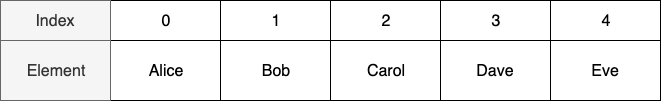
\includegraphics[width=\linewidth, keepratio]{chapters/07_python2_basics/figures/0-based-indexing.png}
                   \caption{Indizierung einer Liste mit 5 Elementen}
               \end{figure}
               
               Im Beispiel hat also das erste Element "Alice" den Index 0 und das letzte Element "Eve" den Index 4.
            \end{alertblock}
        \end{frame}
        
        \begin{frame}[fragile]{Speichern von Werten (VI)}
            \begin{itemize}
                \item \textbf{extend}: Einer Liste können auch Werte hinzugefügt werden, indem die Werte einer weiteren Liste angehängt werden. Hierzu kann die \code{extend()}-Funktion genutzt werden. Die Syntax ist: \\~\
                
                \code{<Liste>.extend(<Liste>)}
                
\begin{pyconcode}
>>> names = ['Alice', 'Bob' 'Carol']
>>> print(names)
['Alice', 'Bob', 'Carol']
>>> names.extend(['Dave', 'Eve'])
>>> print(names)
['Alice', 'Bob', 'Carol', 'Dave', 'Eve']
\end{pyconcode} 

            
            Mit \code{extend()} werden alle Elemente der zweiten Liste ans Ende der ersten Liste angehängt.
            \end{itemize}
        \end{frame}
        
        
        \begin{frame}[fragile]{Auslesen von Werten (I)}
            Um eine Liste sinnvoll nutzen zu können, ist es nicht nur wichtig, Werte in einer Liste abzuspeichern, sondern diese darüber hinaus auch wieder auslesen ("abfragen") zu können. \\~\
            
            Ebenso wie die Erzeugung einer Liste erfolgt die Abfrage eines Elements der Liste durch eckige Klammern, die den jeweiligen Index des gewünschten Elements einschließen. \\~\

\begin{pyconcode}
>>> names = ['Alice', 'Bob', 'Carol', 'Dave']
>>> second_name = names[1]
>>> print(second_name)
'Bob'
\end{pyconcode}             
        
            Hier wird das Element mit dem Index \texttt{1} aus der Liste \code{names} ausgelesen und in der Variablen \code{second\_name} gespeichert. Da die Indizierung 0-basiert ist, ist das Element mit dem Index \texttt{1} \textit{Bob} und nicht \textit{Alice}.
        \end{frame}
        
        \begin{frame}[fragile]{Auslesen von Werten (II)}
            \begin{alertblock}{Achtung}
                Der Programmierer muss stets darauf achten, einen validen Index anzugeben. Übersteigt der Index bspw. die Anzahl der in der Liste enthaltenen Elemente, erscheint ein Fehler

\begin{pyconcode}
>>> names = ['Alice', 'Bob', 'Carol', 'Dave']
>>> names[4]
IndexError: list index out of range
\end{pyconcode}  


            \end{alertblock}
        \end{frame}
        
        \begin{frame}[fragile]{Auslesen von Werten (III)}
            Die Abfrage von Werten mithilfe von Indizes kann auch mit negativen Indizes erfolgen. Hierdurch kann die Liste in umgekehrter Reihenfolge abgefragt werden. Dies macht beispielsweise das Auslesen des letzten Listenelements sehr bequem.

\begin{pyconcode}
>>> names = ['Alice', 'Bob', 'Carol', 'Dave']
>>> last_name = names[-1]
>>> print(last_name)
'Dave'
>>> names[1] == names[-3]
True
\end{pyconcode}  

        \begin{alertblock}{Achtung}
            Das letzte Listenelement besitzt den Index \texttt{-1} und nicht \texttt{-0}, da \texttt{-0} identisch zur Zahl \texttt{0} ist und daher schon für das erste Listenelement vergeben ist
        \end{alertblock}
        
        \end{frame}
        
        
        \begin{frame}[fragile]{Auslesen von Werten (IV)}
            Anstatt einzelner Elemente können auch Bereiche innerhalb einer Liste abgefragt werden. Hierfür wird das sogenannte \textbf{Slicing} genutzt. Die Syntax ist Ähnlich zur Abfrage einzelner Werte, jedoch wird hier ein Bereich von Indizes, getrennt durch \code{:} angegeben.
            
\begin{pyconcode}
>>> names = ['Alice', 'Bob', 'Carol', 'Dave', 'Eve']
>>> names[1:3]
['Bob', 'Carol']
>>> names[0:4]
['Alice', 'Bob', 'Carol', 'Dave']
\end{pyconcode}
        
        Die erste Zahl stellt dabei den Index dar, bei dem gestartet wird (inklusive), die zweite Zahl stellt den Endindex (exklusive) dar. Im 1. Beispiel wird also bei Index 1 ('Bob') begonnen und bei Index 3 ('Dave') gestoppt, da der Endindex jedoch exklusiv ist, werden lediglich Index 1 und 2 berücksichtigt.
        \end{frame}
        
        \begin{frame}[fragile]{Auslesen von Werten (IV)}
            Das Slicing kann noch um einen weiteren Wert, den \textbf{Step} erweitert werden. Indem neben Start und Stop ein dritter Wert angegeben wird, kann bestimmt werden, in welcher Schrittgröße die Elemente aus der Liste gelesen werden sollen. Wird kein Step angegeben (wie im vorherigen Beispiel), wird standardmäßig eine Schrittweite von 1 verwendet.
            
\begin{pyconcode}
>>> numbers = [0, 1, 2, 3, 4, 5, 6, 7]
>>> numbers[1:6:2]
[1, 3, 5]
\end{pyconcode}
        
        Es wird also der Bereich zwischen den Indizes 1 (inklusiv) und 6 (exklusiv) betrachtet und hiervon wird jede 2. Zahl berücksichtigt. Beginnend mit der 1 folgt dann die Zahl 3 sowie die Zahl 5. 
        
        \end{frame}
        
        \begin{frame}[fragile]{Auslesen von Werten (IV)}
            
            Wird kein Start-Index angegeben, wird automatisch bei Index 0 begonnen. Wird kein Stopindex angegeben, wird automatisch beim letzten Index gestoppt. Daher ist z.B. auch folgende Schreibweise denkbar:

 \begin{pyconcode}
>>> numbers = [0, 1, 2, 3, 4, 5, 6, 7]
>>> numbers[3:]
[3, 4, 5, 6, 7]
>>> numbers[:-2]
[0, 1, 2, 3, 4, 5]
>>> numbers[::2]
[0, 2, 4, 6]
\end{pyconcode}   
           Im ersten Beispiel werden alle Elemente beginnend beim 3. Index bis zum Ende der Liste (da kein Endindex angegeben ist) abgefragt (Schrittweite 1).
           
           Im zweiten Beispiel werden alle Elemente beginnend beim Anfang der Liste (da kein Startindex angegeben ist) bis zum vorvorletzten Element abgefragt (Schrittweite 1).
           
           Im dritten Beispiel werden alle Elemente beginnend beim Anfang der Liste (da kein Startindex angegeben ist) bis zum letzten Element (da kein Endindex angegeben ist) in 2-er Schritten abgefragt (\textit{jedes 2. Element der Liste})
          
        \end{frame}
        
         \begin{frame}[fragile]{Auslesen von Werten (IV)}
        
            Mithilfe von Slicing kann bspw. auch ganz einfach die Reihenfolge einer Liste umgekehrt werden:
 
 \begin{pyconcode}
>>> numbers = [0, 1, 2, 3, 4, 5, 6, 7]
>>> numbers[::-1]
[7, 6, 5, 4, 3, 2, 1, 0]
\end{pyconcode}         

        Hier wird vom Anfang der Liste bis zum Ende der Liste in Schritten der Größe \textit{-1}, also rückwärts, gegangen.
            
        \end{frame}
        
        \begin{frame}[fragile]{Löschen von Werten (I)}
            Neben der Möglichkeit, Werte zu einer Liste hinzuzufügen, können die Werte auch wieder gelöscht/entfernt werden, da Listen generell veränderbar sind. \\~\
            
            Auch hierfür stehen unterschiedliche Möglichkeiten zur Verfügung
        \end{frame}
        
        \begin{frame}[fragile]{Löschen von Werten (II)}
            \begin{itemize}
                \item \texttt{delete}-Operator: Um ein Element aus der Liste zu Löschen kann der \texttt{delete}-Operator genutzt werden. Hierfür steht das Schlüsselwort \code{del} zur Verfügung.  Die Syntax ist: \\~\
                
                \code{del <Liste>[<Index>]}
                
\begin{pyconcode}
>>> names = ['Alice', 'Bob', 'Carol', 'Dave']
>>> del names[0]
>>> print(names)
['Bob', 'Carol', 'Dave']
>>> del names[-1]
['Bob', 'Carol']
\end{pyconcode} 

            \end{itemize}
        \end{frame}
        
        
        \begin{frame}[fragile]{Löschen von Werten (III)}
            \begin{itemize}
                \item \textbf{pop}: Mithilfe der \code{pop()}-Funktion wird das Element entsprechend des übergebenen Indizes aus der Liste gelöscht und zurückgegeben. Wird kein Index explizit angegeben, wird das letzte Element der Liste gelöscht und zurückgegeben. Die Syntax ist: \\~\
                
                \code{<Liste>.pop()} bzw. \code{<Liste>.pop(<Index>)}
                
\begin{pyconcode}
>>> names = ['Alice', 'Bob', 'Carol', 'Dave']
>>> names.pop()
'Dave'
>>> print(names)
['Alice', 'Bob', 'Carol']
>>> names.pop(1)
Bob
>>> print(names)
['Alice', 'Carol']
\end{pyconcode} 

            \end{itemize}
        \end{frame}
        
        
        \begin{frame}[fragile]{Löschen von Werten (IV)}
            \begin{itemize}
                \item \textbf{remove}: Mithilfe der \code{remove()}-Funktion wird das erste Element aus der Liste gelöscht, das dem übergebenen Element entspricht. Ebenso wie bei der Abfrage von Werten muss stets darauf geachtet werden, ob der Wert überhaupt in der Liste enthalten ist, da ansonsten ein Fehler auftritt. Die Syntax ist: \\~\
                
                \code{<Liste>.remove(<Element>)}
                
\begin{pyconcode}
>>> names = ['Alice', 'Bob', 'Carol', 'Dave']
>>> names.remove('Bob')
>>> print(names)
['Alice', 'Carol', 'Dave']
>>> names.remove('Bob')
ValueError: list.remove(x): x not in list
\end{pyconcode} 

            \end{itemize}
        \end{frame}
        
        
        \begin{frame}[fragile]{in-Keyword}
            Um zu überprüfen, ob sich ein bestimmter Wert in einer Liste befindet (z.B. bevor die \code{remove()}-Funktion ausgeführt wird), gibt es in Python das Schlüsselwort \code{in}. 
            
            Die Auswertung ist dabei stets ein boolescher Wert: Falls das jeweilige Element in der Liste enthalten ist, wird \code{True} zurückgegeben, andernfalls \code{False}. 
            
            Die Syntax ist: \\~\
            
            \code{<Element> in <Liste>}
            
\begin{pyconcode}
>>> names = ['Alice', 'Bob', 'Carol', 'Dave']
>>> 'Bob' in names
True
>>> names.remove('Bob')
>>> print(names)
['Alice', 'Carol', 'Dave']
>>> 'Bob' in names
False
\end{pyconcode} 

        \end{frame}
        
        
        \begin{frame}[fragile]{Elementanzahl (I)}
            Um zu überprüfen, wie viele Elemente in einer Liste enthalten sind, kann die \code{len()}-Funktion genutzt werden. Diese gibt an, wie viele Werte insgesamt in der Liste gespeichert sind, es handelt sich also immer um einen Integer-Wert. 
            
            Die Syntax ist: \\~\
            
            \code{len(<Liste>)}
            
\begin{pyconcode}
>>> names = ['Alice', 'Bob', 'Carol', 'Dave']
>>> len(names)
4
>>> names.remove('Bob')
>>> print(names)
['Alice', 'Carol', 'Dave']
>>> len(names)
3
\end{pyconcode} 

        \end{frame}
        
        \begin{frame}[fragile]{Elementanzahl (II)}
            
            \begin{alertblock}{Achtung}
                Im Gegensatz zur mathematischen Zählweise bei der Indizierung wird bei der reinen Anzahl der Elemente die natürliche Zählweise genutzt. Wenn also in einer Liste 4 Elemente enthalten sind, ist die Anzahl der Elemente, die durch \code{len()} ermittelt wird, 4 und nicht 3. \\~\
                
                Dies führt in Kombination mit der Indizierung häufig zu Verwirrung und stellt eine häufige Fehlerursache dar.
            \end{alertblock}
        \end{frame}
        
        \begin{frame}[fragile]{Hilfreiche Funktionen (I)}
            
            Da Listen universell und flexibel einsetzbar sind, besitzen sie viele Hilfsfunktionen, die bereits in Python eingebaut sind und ohne weiteres vom Entwickler genutzt werden können. \\~\
            
            Eine Auswahl dieser Hilfsfunktionen wird im Folgenden vorgestellt, ein Überblick über alle Listenfunktionen gibt die \href{https://docs.python.org/3/tutorial/datastructures.html#more-on-lists}{offizielle Dokumentation}.
            
        \end{frame}
        
         \begin{frame}[fragile]{Hilfreiche Funktionen (II)}
            \begin{itemize}
                \item \textbf{sort}: Mithilfe der \code{sort()}-Funktion können Listen sortiert werden. 
                
                Die Syntax ist: \\~\
                
                \code{<Liste>.sort()} \\~\
                
                Sind in der Liste lediglich numerische Werte enthalten, so wird die Liste standardmäßig nach aufsteigende Werte sortiert:
                
\begin{pyconcode}
>>> numbers = [3, 6, 1, 9, 18, 4]
>>> numbers.sort()
>>> print(numbers)
[1, 3, 4, 6, 9, 18]
\end{pyconcode} 
            \end{itemize}
         \end{frame}
         
         \begin{frame}[fragile]{Hilfreiche Funktionen (III)}
            
            Sind in der Liste lediglich Strings enthalten, so wird die Liste standardmäßig alphabetisch aufsteigend sortiert:

\begin{pyconcode}
>>> addresses = ['Palm Springs 210', 'Sunset Blvd. 10', 'Eastriver Drive 50', '11th Street 09']
>>> addresses.sort()
>>> print(addresses)
['11th Street 09', 'Eastriver Drive 50', 'Palm Springs 210', 'Sunset Blvd. 10']
\end{pyconcode} 

             Sind in der Liste unterschiedliche Datentypen enthalten, so kann die Liste nicht sortiert werden, da unklar ist, wie etwa Strings und Integer-Werte miteinander verglichen werden sollen \footnote{In diesen Fällen kann der Entwickler eine eigene Vergleichs-/Sortierfunktion angeben}:

\begin{pyconcode}
>>> names_and_ages = ['Alice', 23, 'Bob', 21, 'Carol', 34, 'Dave', 19]
>>> names_and_ages.sort()
TypeError: '<' not supported between instances of 'int' and 'str'
\end{pyconcode} 

         \end{frame}
         
         
         \begin{frame}[fragile]{Hilfreiche Funktionen (IV)}
            
            Die Listen können auch absteigend sortiert werden, indem der Parameter \code{reverse=True} mit übergeben wird:
            
\begin{pyconcode}
>>> numbers = [3, 6, 1, 9, 18, 4]
>>> numbers.sort(reverse=True)
>>> print(numbers)
[18, 9, 6, 4, 3, 1]
\end{pyconcode} 

         \end{frame}
         
         
         \begin{frame}[fragile]{Hilfreiche Funktionen (V)}
            \begin{itemize}
                \item \textbf{reverse}: Analog zum Sortieren kann die Reihung der Elemente innerhalb einer Liste auch invertiert werden, die Liste wird also "umgedreht". Hierfür gibt es die \code{reverse()}-Funktion.
                
                Die Syntax ist: \\~\
                
                \code{<Liste>.reverse()}

\begin{pyconcode}
>>> names = ['Alice', 'Bob', 'Carol', 'Dave']
>>> names.reverse()
>>> print(names)
['Dave', 'Carol', 'Bob', 'Alice']
\end{pyconcode} 

            \end{itemize}
            
        \end{frame}
        
         \begin{frame}[fragile]{Hilfreiche Funktionen (VI)}
            \begin{itemize}
                \item \textbf{min/max/sum}: Auch mathematische Funktionen, die auf Listen angewandt werden können, sind vorhanden.
                
\begin{pyconcode}
>>> numbers = [3, 6, 1, 9, 18, 4]
>>> max(numbers)
18
>>> min(numbers)
1
>>> sum(numbers)
41
\end{pyconcode} 


            \end{itemize}
         \end{frame}
         
    
    \begin{subsubsection}{Aufgaben}
        \begin{frame}[allowframebreaks]{Aufgaben}
            \begin{enumerate}
                \item Was sind Listen? Wofür werden sie genutzt? Was ist der Vorteil ggü. zuvor besprochener Datentypen?
                \item Welche Eigenschaften besitzt eine Liste und was bedeuten diese?
                \item Wie können Listen erzeugt werden?
                \item Erzeugen Sie eine vorgefüllte Liste mit den Werten \texttt{1}, \texttt{3}, \texttt{5} und \texttt{7}
                \item Fügen sie dieser Liste den Wert \texttt{9} an
                \item Wie können mehrere Werte auf einmal angehängt werden? Fügen Sie die Werte \texttt{11}, \texttt{13} und \texttt{17} in einem Schritt an.
                \item Da der Wert \texttt{15} ausgelassen wurde, soll dieser nun ebenfalls zur Liste hinzugefügt werden, sodass die Sortierung der Werte intakt bleibt.
                \item Gegeben ist \code{x = [3,5,1,2,4,6]}. Welchen Wert hat \code{x[2]}? Welchen \code{x[-2]}?
                \item Mit welchem Befehl können in der zuvor erzeugten Liste der ungeraden Zahlen die Zahlen von 5 - 13 abgefragt werden?
                \item Wie kann diese Liste invertiert werden?
                \item Wie kann jeder dritte Wert dieser Liste abgefragt werden?
                \item Worin besteht der Unterschied zwischen \texttt{del}, \texttt{pop} und \texttt{remove}?
                \item Was ist das Ergebnis von \code{[1,1,2,2,3,3].remove(2)}?
                \item Wofür wird das \code{in}-Keyword genutzt? Was muss bei der Verwendung von Keywords beachtet werden?
                \item Worauf muss bei der Indizierung und der Längenangaben von Listen geachtet werden?
                \item Welche weitere Möglichkeit gibt es, die Reihenfolge einer Liste (permanent) umzukehren?
                \item Was ist das Ergebnis?: \code{max(['Bert', 'cArl', 'adam'])}
            \end{enumerate}
        \end{frame}
    \end{subsubsection}
    
    \begin{subsection}{Tuples}
    
        \begin{frame}{Tuples - Definition}
            Neben den Listen existiert ein weiterer häufig verbreiteter Sequenzdatentyp in Python: Das Tuple. Ein Tuple verhält sich sehr ähnlich zu einer Liste.
            
            \begin{block}{Tuple}
                Ein Tuple ist eine unveränderbare, geordnete und indizierte Sammlung von Objekten
            \end{block}
            
            Der primäre Unterschied zu Listen besteht also darin, dass Tuples unveränderbar sind, Werte können also nicht überschrieben und bestehende Tuples nicht abgeändert werden.
        \end{frame}
        
        \begin{frame}{Einsatz von Tuples}
            Ebenso wie Listen können auch in einem Tuple unterschiedliche Datentypen enthalten sein. \\~\
            
            Aufgrund der Unveränderbarkeit der Werte werden Tuples häufig als Rückgabewerte von Funktionen genutzt, sofern mehrere Werte zurückgegeben werden sollen.
        \end{frame}
        
        \begin{frame}[fragile]{Erzeugung (I)}
            Ein Tuple kann auf unterschiedliche Arten erzeugt werden: \\~\
            
            \begin{itemize}
                \item \code{tuple()}-Konstruktor: Mithilfe des Befehls \code{tuple()} kann ein neues, zunächst leeres Tuple erzeugt werden.
                
\begin{pyconcode}
>>> new_tuple = tuple()
>>> print(new_tuple)
()
>>> type(new_tuple)
<class 'tuple'>
\end{pyconcode}                 
            \end{itemize}
        \end{frame}
        
        \begin{frame}[fragile]{Erzeugung (II)}
            
            \begin{itemize}
                \item Kurzschreibweise: Elemente, die in einem Tuple enthalten sind, werden in Python durch runde Klammern (\code{( )}) umgeben. Als Kurzschreibweise kann anstatt \code{tuple()} daher auch einfach \code{()} genutzt werden.
                
\begin{pyconcode}
>>> new_tuple = ()
>>> print(new_tuple)
()
>>> type(new_tuple)
<class 'tuple'>
\end{pyconcode}                 
            \end{itemize}
        \end{frame}
        
        
        \begin{frame}[fragile]{Speichern von Werten (I)}
            
          In den beiden vorherigen Beispielen wurde gezeigt, wie Tuples erzeugt werden können, jedoch enthalten diese Tuples noch keine Werte, sind also \textit{leer}. Um Werte in den Tuples abzuspeichern gibt es die Möglichkeit, Werte direkt bei der Erzeugung anzugeben.
        \end{frame}
        
         \begin{frame}[fragile]{Speichern von Werten (II)}
         
         \begin{itemize}
             \item \textbf{Erzeugung eines vorgefüllten Tuples:} Bei der Initialisierung eines neuen Tuples können direkt Objekte angegeben werden, die in diesem Tuple gespeichert werden sollen: 

\begin{pyconcode}
>>> names = ('Alice', 'Bob', 'Carol', 'Dave')
>>> print(names)
('Alice', 'Bob', 'Carol', 'Dave')
>>> type(names)
<class 'tuple'>
\end{pyconcode}  
    
            Bei der Erzeugung von Tuples können die Klammern auch weggelassen werden. Jedoch sollten sie aus Gründen der Übersichtlichkeit immer genutzt werden.
            
\begin{pyconcode}
>>> names = 'Alice', 'Bob', 'Carol', 'Dave'
>>> type(names)
<class 'tuple'>
\end{pyconcode}  


         \end{itemize}
        \end{frame}
        
        \begin{frame}[fragile]{Speichern von Werten (III)}
            
            Soll ein Tuple mit lediglich einem Wert angelegt werden, ist das Komma trotzdem notwendig, um zwischen einer einfachen Wertzuweisung und einer Erzeugung eines Tuples unterscheiden zu können.
    
\begin{pyconcode}
>>> name_without_comma = ('Alice')
>>> name_with_comma = ('Alice',)
>>> type(name_without_comma)
<class 'str'>
>>> type(name_with_comma)
<class 'tuple'>
\end{pyconcode}  
        \end{frame}
        
        \begin{frame}[fragile]{Speichern von Werten (IV)}
         
            \begin{alertblock}{Achtung}
                Das gleichzeitige Erzeugen eines Tuples und Speichern von Werten in ebendiesem Tuple ist nur mit der Kurzschreibweise möglich. Wird ein Tuple mit tuple() erzeugt, können die Werte nicht direkt im Tuple gespeichert werden, auch ein späteres Hinzufügen ist nicht möglich (da Tuples unveränderbar sind).
            \end{alertblock}
        \end{frame}
        
        
        \begin{frame}[fragile]{Speichern von Werten (V)}
            \begin{alertblock}{Achtung}
               Funktionen wie \code{append()}, \code{insert()} oder \code{extend()} sind bei Tuples nicht vorhanden, da Tuples grundsätzlich unveränderbar sind.
            \end{alertblock}
        \end{frame}
      
        \begin{frame}[fragile]{Tuple-Operationen (I)}
           Es können verschiedene Operationen verwendet werden, um neue Tuple zu erzeugen: \\~\
           
           \begin{itemize}
               \item \textbf{Tuple Konkatenation}: Mithilfe des \code{+}-Operators können zwei Tuple konkateniert (verbunden) werden. Da die Tuple unveränderbar sind, entsteht dadurch ein neues, drittes Tuple

\begin{pyconcode}
>>> names1 = ('Alice', 'Bob')
>>> names2 = ('Carol', 'Dave')
>>> names3 = names1 + names2
>>> print(names3)
('Alice', 'Bob', 'Carol', 'Dave')
>>> type(names3)
<class 'tuple'>
\end{pyconcode}                 
               
           \end{itemize}
        \end{frame}
        
        
        \begin{frame}[fragile]{Tuple-Operationen (II)}

           \begin{itemize}
               \item \textbf{Multiple Konkatenation}: Mithilfe des \code{*}-Operators kann der Inhalt eines Tuples beliebig oft wiederholt werden. Da das Tuple unveränderbar ist, entsteht dadurch ein neues Tuple

\begin{pyconcode}
>>> names1 = ('Alice', 'Bob')
>>> names2 = names1 * 4
>>> print(names2)
('Alice', 'Bob', 'Alice', 'Bob', 'Alice', 'Bob', 'Alice', 'Bob')
>>> type(names2)
<class 'tuple'>
\end{pyconcode}                 
               
           \end{itemize}
        \end{frame}
        
        
        \begin{frame}[fragile]{Auslesen von Werten}
            Das Auslesen der Tuple-Werte verhält sich identisch zum Auslesen von Werten aus Listen. \\~\
            
            \begin{alertblock}{Achtung}
                Auch wenn Tuples mit runden Klammern erzeugt werden, erfolgt das Auslesen von Werten (wie bei allen Sequenz-Typen) mit eckigen Klammern!
            \end{alertblock}
            
            Auch Tuples sind indexbasiert, die wieder 0-basiert sind. Es muss auch beachtet werden, dass der Tuple-Index bei der Abfrage nicht größer ist als die Länge des Tuples
            
\begin{pyconcode}
>>> names = ('Alice', 'Bob', 'Carol', 'Dave')
>>> print(names[1])
'Bob'
>>> print(names[4])
IndexError: tuple index out of range
>>> print(names[-1])
'Dave'
\end{pyconcode}                 
               
                           
        \end{frame}
        
        
        \begin{frame}[fragile]{Löschen von Werten}
            Da Tuples unveränderlich sind, können Werte aus einem Tuple nicht entfernt werden. Wird trotzdem versucht, einen Wert zu löschen, erscheint ein Fehler:
            
\begin{pyconcode}
>>> names = ('Alice', 'Bob', 'Carol', 'Dave')
>>> del names[0]
TypeError: 'tuple' object doesn't support item deletion
\end{pyconcode}                 
        
        Soll trotzdem ein Wert aus einem Tuple gelöscht werden, kann dies über einen Workaround gelöst werden: Es kann ein neues Tuple, bestehend aus den Werten des alten Tuples exklusive des zu löschenden Wertes, erzeugt werden:

\begin{pyconcode}
>>> names = ('Alice', 'Bob', 'Carol', 'Dave')
>>> names_without_bob = (names[0],) + names[2:]
>>> print(names_without_bob)
('Alice', 'Carol', 'Dave')
\end{pyconcode}     
                           
        \end{frame}
        
        
         \begin{frame}[fragile]{in-Keyword}
            Ebenso wie bei den Listen kann mithilfe des \code{in}-Keywords festgestellt werden, ob ein Wert in einem Tuple enthalten ist.
            
\begin{pyconcode}
>>> names = ('Alice', 'Bob', 'Carol', 'Dave')
>>> 'Bob' in names
True
\end{pyconcode}                 
        
        \end{frame}
        
        
        \begin{frame}[fragile]{Elementzahl}
            Ebenso wie bei den Listen kann mithilfe der \code{len()}-Funktion festgestellt werden, wie viele Werte in einem Tuple enthalten sind.
            
\begin{pyconcode}
>>> names = ('Alice', 'Bob', 'Carol', 'Dave')
>>> len(names)
4
\end{pyconcode}                 
        
        \end{frame}
        
        
        \begin{frame}[fragile]{Hilfreiche Funktionen}
            Da Tuples unveränderbar sind, stehen hier keine der Funktionen zur Verfügung, die die Struktur der Tuples direkt verändern (z.B. \code{sort()}, \code{reverse()}, ...). \\~\
            
            Dennoch gibt es auch hier Tuple-Funktionen, die die Struktur nicht beeinflussen, wie etwa \code{min()}, \code{max()}, \code{sum()},...
            
\begin{pyconcode}
>>> ages = (23, 52, 21, 33)
>>> max(ages)
52
>>> sum(ages)
129
\end{pyconcode}                 
        
        \end{frame}
        
        
    
        \begin{subsubsection}{Aufgaben}
             \begin{frame}[allowframebreaks,fragile]{Aufgaben}
                \begin{enumerate}
                    \item Worin besteht der primäre Unterschied zwischen Listen und Tuples?
                    \item Wann werden Listen verwendet? Wann Tuples?
                    \item Welche Möglichkeiten gibt es, ein Tuple mit Werten zu füllen?
                    \item Welchen Zweck erfüllt der Tuple-Konstruktor?
                    \item Mit welchen der folgenden Ausdrücke wird ein Tuple erzeugt? Was ist jeweils das Ergebnis von \code{i[0]}?:
                        \begin{itemize}
                            \item
\begin{pyconcode}
>>> i = 0
>>> i[0]
\end{pyconcode}    
                            \item
\begin{pyconcode}
>>> i = (0)
>>> i[0]
\end{pyconcode}  
                            \item
\begin{pyconcode}
>>> i = (0),
>>> i[0]
\end{pyconcode}   
                            \item
\begin{pyconcode}
>>> i = (0,)
>>> i[0]
\end{pyconcode}   
                            \item
\begin{pyconcode}
>>> i = (0,),
>>> i[0]
\end{pyconcode}   
                            \item
\begin{pyconcode}
>>> i = 0,
>>> i[0]
\end{pyconcode}    
                            \item
\begin{pyconcode}
>>> i = "0"
>>> i[0]
\end{pyconcode}   
                           \item
\begin{pyconcode}
>>> i = "0,"
>>> i[0]
\end{pyconcode}   
                        \end{itemize}
                    \item Was ist bei Tuples bezüglich Kommas und Klammern zu beachten?
                    \item Wie kann dem Tuple \code{('Alice','Bob')} der Wert \code{'Carol'} angehängt werden?
                    \item Welche Ausgabe erzeugt folgender Befehl?:

\begin{pyconcode}
>>> tuple1 = ('na',)
>>> tuple2 = 'Batman',
>>> tuple1*10 + tuple2
\end{pyconcode}                     
                    \item Für den Zugriff auf Tuplewerte durch Indizes werden eckige Klammern verwendet. Warum werden diese nicht auch zur Erzeugung eines Tuples verwendet?
                    
                    \item Wie können Werte aus einem Tuple gelöscht werden? Was ist dabei zu beachten?
                    
                    \item Welche Funktionen sind bei Listen und Tuples anwendbar, welche lediglich bei Listen? Warum gilt diese Einschränkung?
                \end{enumerate}
            \end{frame}
        \end{subsubsection}
    \end{subsection}
    
    \begin{subsection}{Dictionaries}
    
        \begin{frame}{Dictionaries - Definition}
            Zu den erweiterten Grunddatentypen gehören bei Python auch die sogenannten \textit{Dictionaries}, die im deutschen auch seltener als \textit{Wörterbücher} bezeichnet werden.
            
            \begin{block}{Dictionary}
                Ein Dictionary ist eine veränderbare ungeordnete Sammlung von Werten in einer Key-Value Struktur
            \end{block}
        \end{frame}
    
        \begin{frame}{Key-Value Struktur}
            Eine \textit{Key-Value Struktur} ist eine in der Programmierung häufig genutzte Struktur, um eindeutige Relationen zwischen einem Schlüsselwert (\textbf{Key}) und einer entsprechenden Wertzuweisung (\textbf{Value}) herzustellen. \\~\
            
            \begin{exampleblock}{Beispiel}
                \textbf{Relation Länder \textrightarrow Hauptstädte:}
                
                \textit{"Deutschland"} \textrightarrow \textit{"Berlin"}, \textit{"Frankreich"} \textrightarrow \textit{"Paris"}, \textit{"Italien"} \textrightarrow \textit{"Rom"}, ... \\~\
                
                \textbf{Relation Name \textrightarrow Körpergröße:}
                
                \textit{"Alice"} \textrightarrow \textit{179}, \textit{"Bob"} \textrightarrow \textit{181}, \textit{"Eve"} \textrightarrow \textit{165}, ...\\~\
                
                \textbf{Relation Smarthome-Element \textrightarrow Zustand:}
                
                \textit{"Licht an"} \textrightarrow \textit{True}, \textit{"Fenster offen"} \textrightarrow \textit{False}, \textit{"Türe geschlossen"} \textrightarrow \textit{True}, ...
                

            \end{exampleblock}
        \end{frame}
        
        \begin{frame}{Eigenschaften}
            Ebenso wie Listen und im Gegensatz zu Tuples sind Dictionaries veränderbar, d.h. Werte innerhalb der Dictionaries können überschrieben und die Struktur der Dictionaries verändert werden, ohne dafür explizit ein neues Objekt erzeugen zu müssen. \\~\
            
            Im Gegensatz zu Listen und Tuples sind Dictionaries ungeordnet, d.h. die Elemente liegen nicht zwingend in der Reihenfolge vor, in der sie angelegt wurden. \footnote{Erst ab Python 3.7 sind Dictionaries immer \textit{insertion-ordered}}
            
            Da Dictionaries im Gegensatz zu den Sequence-Types nicht indexbasiert, sondern keybasiert ist, ist die Reihenfolge in den meisten Fällen irrelevant.
            
        \end{frame}
        
        \begin{frame}{Eigenschaften von Keys und Values}
            Die Keys und Values eines Dictionaries müssen gewisse Eigenschaften erfüllen:\\~\
            
            \begin{itemize}
                \item \textbf{Keys:}
                    \begin{itemize}
                        \item \textbf{Uniqueness:} Keys müssen \textit{unique} (eindeutig) sein. Es darf kein Wert mehrmals als Key innerhalb eines Dictionaries verwendet werden
                        \item \textbf{Hashable:} Keys müssen \textit{immutable} (unveränderbar) sein. Basisdatentypen (int, float, string, ...) sind also erlaubt, ebenso reine Tuples. Listen und Dictionaries sind veränderbar, daher können sie nicht als Key genutzt werden.
                        \item \textbf{Numerische Gleichheit:} Sofern zwei Zahlen als \textit{gleich} betrachtet werden, verweisen sie auf den selben Key (Bsp.: Da in Python gilt \code{1 == 1.0}, stellen beide Zahlen den gleichen Key dar)
                    \end{itemize}
                \item \textbf{Values:}
                    \begin{itemize}
                        \item Annähernd alle Objekte und Datentypen dürfen als Values innerhalb eines Dictionaries verwendet werden, z.B. Grunddatentypen (int, float, string, ...), erweiterte Datentypen (Sequenzen (Listen, Tuples), Maps (Dictionaries), Sets), Klassen, Objekte, ...
                    \end{itemize}
            \end{itemize}
        \end{frame}
        
        \begin{frame}[fragile]{Erzeugung (I)}
            Ein Dictionary kann auf unterschiedliche Arten erzeugt werden:
            
            \begin{itemize}
                \item \code{dict()}-Konstruktor: Mithilfe des Befehls \code{dict()} kann ein neues, zunächst \textit{leeres} Dictionary erzeugt werden
            \end{itemize}

\begin{pyconcode}
>>> new_dictionary = dict()
>>> print(new_dictionary)
{}
>>> type(new_dictionary)
<class 'dict'>
\end{pyconcode}             
    
        \end{frame}
        
        \begin{frame}[fragile]{Erzeugung (II)}
            
            \begin{itemize}
                \item Kurzschreibweise: Elemente, die in einem Dictionary enthalten sind, werden in Python durch geschweifte Klammern (\code{\{ \}}) umgeben. Als Kurzschreibweise kann anstatt \code{dict()} daher auch einfach \code{\{\}} genutzt werden
            \end{itemize}

\begin{pyconcode}
>>> new_dictionary = {}
>>> print(new_dictionary)
{}
>>> type(new_dictionary)
<class 'dict'>
\end{pyconcode}             
    
        \end{frame}

        
        \begin{frame}[fragile]{Speichern von Werten (I)}
            
            In beiden vorherigen Beispielen wurde gezeigt, wie Dictionaries erzeugt werden können, jedoch enthalten diese Dictionaries noch keine Werte, sind also \textit{leer}. Um Werte in den Listen abzuspeichern, gibt es unterschiedliche Möglichkeiten.
    
        \end{frame}
    
        \begin{frame}[fragile]{Speichern von Werten (II)}
            
           \begin{itemize}
               \item \textbf{Erzeugung eines vorgefüllten Dictionaries:} Bei der Initialisierung eines neuen Dictionaries können direkt Objekte angegeben werden, die in diesem Dictionary gespeichert werden sollen:

\begin{pyconcode}
>>> capitals = {'Germany': 'Berlin', 'France': 'Paris', 'Italy': 'Rome'}
>>> print(capitals)
{'Germany': 'Berlin', 'France': 'Paris', 'Italy': 'Rome'}
>>> type(capitals)
<class 'dict'>
\end{pyconcode}

            Hier wird ein Dictionary erzeugt, das jeweils einem Land (Key) eine Hauptstadt (Value) zuweist. Die Syntax eines Dictionaries sieht folgendermaßen aus: \\~\
            
            \code{\{<Key>: <Value>, <Key>: <Value>, ...\}}
            
            Einzelne Einträge werden also durch Komma getrennt, Values werden den Keys durch Doppelpunkt zugewiesen.

           \end{itemize}
    
        \end{frame}
        
        \begin{frame}[fragile]{Speichern von Werten (III)}
            
          \begin{alertblock}{Achtung}
            Das gleichzeitige Erzeugen eines Dictionaries und Speichern von Werten in ebendiesem Dictionary ist nur mit Kurzschreibweise möglich. Wird ein Dictionary mit \code{dict()} erzeugt, können die Werte nicht direkt im Dictionary gespeichert werden, hierzu ist ein extra Schritt notwendig.
          \end{alertblock}
    
        \end{frame}
        
        
         \begin{frame}[fragile]{Speichern von Werten (IV)}
            
            \begin{itemize}
                \item \textbf{insert:} Anders als bei den Listen gibt es keine dedizierten \code{append()}, \code{insert()}, ... Funktionen, sondern um einen Wert im Dictionary zu ergänzen bzw. zu überschreiben, genügt folgender Wertzuweisung:\\~\
                
                \code{<Dictionary>[<Key>] = <Value>}
                
                Dies entspricht der normalen Wertzuweisung von Variablen.
            
\begin{pyconcode}
>>> capitals = {'Germany': 'Berlin', 'France': 'Paris', 'Italy': 'Rome'}
>>> print(capitals)
{'Germany': 'Berlin', 'France': 'Paris', 'Italy': 'Rome'}
>>> capitals['Spain'] = 'Barcelona'
>>> print(capitals)
{'Germany': 'Berlin', 'France': 'Paris', 'Italy': 'Rome', 'Spain': 'Barcelona'}
>>> capitals['Spain'] = 'Madrid'
>>> print(capitals)
{'Germany': 'Berlin', 'France': 'Paris', 'Italy': 'Rome', 'Spain': 'Madrid'}
\end{pyconcode}    
                
            \end{itemize}
    
        \end{frame}
        
        \begin{frame}[fragile]{Speichern von Werten (V)}
            
            \begin{itemize}
                \item \textbf{update:} Darüber hinaus existiert auch die \code{update()}-Methode, um Werte dem Dictionary hinzuzufügen bzw. bestehende Werte zu aktualisieren. Die Syntax ist:\\~\
                
                \code{<Dictionary>.update(<Dictionary>)}
                
                Falls das jeweilige Key-Value-Paar im Dictionary bereits vorhanden ist, wird es überschrieben, andernfalls wird es ergänzt.
            
\begin{pyconcode}
>>> capitals = {'Germany': 'Berlin', 'France': 'Paris', 'Italy': 'Rome', 'Spain': 'Barcelona'}
>>> print(capitals)
{'Germany': 'Berlin', 'France': 'Paris', 'Italy': 'Rome', 'Spain': 'Barcelona'}
>>> capitals.update({'Spain':'Madrid', 'Austria': 'Vienna'})
>>> print(capitals)
{'Germany': 'Berlin', 'France': 'Paris', 'Italy': 'Rome', 'Spain': 'Madrid', 'Austria': 'Vienna'}
\end{pyconcode}    
                
            \end{itemize}
    
        \end{frame}
        
        
        \begin{frame}[fragile]{Auslesen von Werten (I)}
            
            Ebenso wie bei Listen und Tuples können Werte aus den Dictionaries mit eckigen Klammern abgefragt werden. Jedoch sind Dictionaries nicht indexbasiert, sondern keybasiert. D.h. auf die jeweiligen Werte kann durch den zugehörigen Key zugegriffen werden.
            
\begin{pyconcode}
>>> capitals = {'Germany': 'Berlin', 'France': 'Paris', 'Italy': 'Rome'}
>>> print(capitals['Germany'])
'Berlin'
\end{pyconcode}    
                
    
        \end{frame}
    
        \begin{frame}[fragile]{Auslesen von Werten (II)}
            
            \begin{alertblock}{Achtung}
                Der Programmierer muss stets darauf achten, einen validen Key anzugeben. Ist der jeweilige Key nicht im Dictionary enthalten, erscheint ein Fehler
                
\begin{pyconcode}
>>> capitals = {'Germany': 'Berlin', 'France': 'Paris', 'Italy': 'Rome'}
>>> print(capitals['Norway'])
KeyError: 'Norway'
\end{pyconcode}    
    
        \end{alertblock}
    
        \end{frame}
        
        \begin{frame}[fragile]{Auslesen von Werten (III)}
            
            \begin{alertblock}{Achtung}
                Im Dictionary können Wert lediglich anhand des Keys abgefragt werden. Eine Abfrage nach Wert ist nicht möglich (Analogie: Wörterbuch)
            
\begin{pyconcode}
>>> capitals = {'Germany': 'Berlin', 'France': 'Paris', 'Italy': 'Rome'}
>>> print(capitals['Berlin'])
KeyError: 'Berlin'
\end{pyconcode}    
                
        \end{alertblock}
        \end{frame}
        
        \begin{frame}[fragile]{Auslesen von Werten (IV)}
            
            Dem Programmierer steht darüber hinaus die \code{get()}-Methode zur Verfügung. Ebenso wie bei der zuvor gezeigten key-basierten Abfrage mithilfe eckiger Klammern können so die Werte zu einem Key abgefragt werden. Außerdem kann ein Default-Wert angegeben werden, der als Ergebnis zurückgegeben wird, falls der Key nicht vorhanden ist.
            
\begin{pyconcode}
>>> capitals = {'Germany': 'Berlin', 'France': 'Paris', 'Italy': 'Rome'}
>>> capital = capitals.get('France')
>>> print(capital)
'Paris'
>>> capital = capitals.get('Norway')
>>> print(capital)
None
>>> capital = capitals.get('Norway', 'nicht enthalten')
>>> print(capital)
'nicht enthalten'
\end{pyconcode}    
                
        
        \end{frame}
    
        \begin{frame}[fragile]{Löschen von Werten (I)}
            
           Neben der Möglichkeit, Werte zu einem Dictionary hinzuzufügen, können die Werte auch wieder gelöscht/entfernt werden, da Dictionaries generell veränderbar sind. \\~\
           
           Auch hierfür stehen unterschiedliche Möglichkeiten zur Verfügung
                
        \end{frame}
        
        \begin{frame}[fragile]{Löschen von Werten (II)}
        
            \begin{itemize}
                \item \texttt{delete}-Operator: Um ein Element aus der Liste zu löschen kann der \texttt{delete}-Operator genutzt werden. Hierfür steht das Schlüsselwort \code{del} zur Verfügung. Die Syntax ist: \\~\
                
                \code{del <Dictionary>[<Key>]}
                
\begin{pyconcode}
>>> capitals = {'Germany': 'Berlin', 'France': 'Paris', 'Italy': 'Rome'}
>>> print(capitals)
{'Germany': 'Berlin', 'France': 'Paris', 'Italy': 'Rome'}
>>> del capitals['Germany']
>>> print(capitals)
{'France': 'Paris', 'Italy': 'Rome'}
\end{pyconcode}  
            \end{itemize}
                
        \end{frame}
        
        \begin{frame}[fragile]{Löschen von Werten (III)}
        
            \begin{itemize}
                \item \textbf{pop}: Mithilfe der \code{pop()}-Methode wird ein Key-Value-Paar anhand des Key-Wertes aus dem Dictionary gelöscht. Zudem wird der Wert des gelöschten Paares zurückgegeben. Die Syntax ist: \\~\
                
                \code{<Dictionary>.pop(<Key>)}
                
\begin{pyconcode}
>>> capitals = {'Germany': 'Berlin', 'France': 'Paris', 'Italy': 'Rome'}
>>> print(capitals)
{'Germany': 'Berlin', 'France': 'Paris', 'Italy': 'Rome'}
>>> removed_capital = capitals.pop('France')
>>> print(removed_capital)
'Paris'
\end{pyconcode}  
            \end{itemize}
                
        \end{frame}
        
        \begin{frame}[fragile]{Löschen von Werten (IV)}
        
            \begin{itemize}
                \item \textbf{popitem}: Mithilfe der \code{popitem()}-Methode wird ein zufälliges Key-Value-Paar aus dem Dictionary gelöscht. Zudem wird das Key-Value-Paar des gelöschten Elements als Tuple zurückgegeben. Die Syntax ist: \\~\
                
                \code{<Dictionary>.popitem()}
                
\begin{pyconcode}
>>> capitals = {'Germany': 'Berlin', 'France': 'Paris', 'Italy': 'Rome'}
>>> print(capitals)
{'Germany': 'Berlin', 'France': 'Paris', 'Italy': 'Rome'}
>>> removed_capital = capitals.popitem()
>>> print(removed_capital)
('Italy', 'Rome')
\end{pyconcode}  
            \end{itemize}
                
        \end{frame}
        
        \begin{frame}[fragile]{Löschen von Werten (V)}
        
            \begin{itemize}
                \item \textbf{clear}: Mithilfe der \code{clear()}-Methode werden alle Key-Value-Paare aus dem Dictionary gelöscht. Die Syntax ist: \\~\
                
                \code{<Dictionary>.clear()}
                
\begin{pyconcode}
>>> capitals = {'Germany': 'Berlin', 'France': 'Paris', 'Italy': 'Rome'}
>>> print(capitals)
{'Germany': 'Berlin', 'France': 'Paris', 'Italy': 'Rome'}
>>> capitals.clear()
>>> print(capitals)
{}
\end{pyconcode}  
            \end{itemize}
                
        \end{frame}
        
        \begin{frame}[fragile]{in-Keyword}
        
            Ebenso wie bei Listen und Tuples, kann das \code{in}-Keyword genutzt werden, um zu überprüfen, ob sich ein Key in einem Dictionary befindet.
                
\begin{pyconcode}
>>> capitals = {'Germany': 'Berlin', 'France': 'Paris', 'Italy': 'Rome'}
>>> 'Italy' in capitals
True
>>> 'Berlin' in capitals
False
\end{pyconcode}  
        
                
        \end{frame}
        
        \begin{frame}[fragile]{Elementanzahl}
        
            Um zu überprüfen, wie viele Key-Value-Paare sich in einem Dictionary befinden, kann die \code{len()}-Funktion genutzt werden.
                
\begin{pyconcode}
>>> capitals = {'Germany': 'Berlin', 'France': 'Paris', 'Italy': 'Rome'}
>>> len(capitals)
3
>>> capitals.clear()
0
\end{pyconcode}  
        
                
        \end{frame}
        
        \begin{frame}[fragile]{Hilfreiche Funktionen (I)}
        
            Da Dictionaries universell und flexibel einsetzbar sind, besitzen sie viele Hilfsfunktionen, die bereits in Python eingebaut sind und ohne weiteres vom Entwickler genutzt werden können.\\~\
            
            Eine Auswahl dieser Hilfsfunktionen wird im Folgenden vorgestellt, ein Überblick über alle Dictionaryfunktionen gibt die \href{https://docs.python.org/3/tutorial/datastructures.html#dictionaries}{offizielle Dokumentation}
                
        \end{frame}
        
        \begin{frame}[fragile]{Hilfreiche Funktionen (II)}
        
            \begin{itemize}
                \item \textbf{items:} Mithilfe der \code{items()}-Methode werden alle Key-Value-Paare in einem sogenannten \textit{View-Objekt}\footnote{View-Objekte stellen eine dynamische Repräsentation der Dictionaries dar. Sie können wie Listen verwendet werden} zurückgegeben. Jedes Key-Value-Paar wird durch ein Tuple repräsentiert. Die Syntax ist: \\~\
                
                \code{<Dictionary>.items()}
  
\begin{pyconcode}
>>> capitals = {'Germany': 'Berlin', 'France': 'Paris', 'Italy': 'Rome'}
>>> items = capitals.items()
>>> print(items)
dict_items([('Germany', 'Berlin'), ('France', 'Paris'), ('Italy', 'Rome')])
\end{pyconcode}                
                
            \end{itemize}
                
        \end{frame}
        
        \begin{frame}[fragile]{Hilfreiche Funktionen (III)}
        
            \begin{itemize}
                \item \textbf{keys:} Mithilfe der \code{keys()}-Methode werden alle Keys des Dictionaries in einem \textit{View-Objekt} zurückgegeben. Die Syntax ist: \\~\
                
                \code{<Dictionary>.keys()}
  
\begin{pyconcode}
>>> capitals = {'Germany': 'Berlin', 'France': 'Paris', 'Italy': 'Rome'}
>>> keys = capitals.keys()
>>> print(keys)
dict_keys(['Germany', 'France', 'Italy'])
\end{pyconcode}                
                
            \end{itemize}
                
        \end{frame}
        
        \begin{frame}[fragile]{Hilfreiche Funktionen (IV)}
        
            \begin{itemize}
                \item \textbf{values:} Mithilfe der \code{values()}-Methode werden alle Values des Dictionaries in einem \textit{View-Objekt} zurückgegeben. Die Syntax ist: \\~\
                
                \code{<Dictionary>.values()}
  
\begin{pyconcode}
>>> capitals = {'Germany': 'Berlin', 'France': 'Paris', 'Italy': 'Rome'}
>>> values = capitals.values()
>>> print(values)
dict_values(['Berlin', 'Paris', 'Rome'])
\end{pyconcode}                
                
            \end{itemize}
                
        \end{frame}
        
        \begin{frame}[fragile]{Hilfreiche Funktionen (V)}
        
             Auf Dictionaries (bzw. deren Werte) können auch Mengenoperationen durchgeführt werden. Die folgenden Beispiele sind jeweils für die \code{items()}-Methode anwendbar. \\~\
            
            \begin{itemize}
                \item \textbf{Schnittmenge:} Mithilfe des \code{\&}-Operators können Schnittmengen zwischen Dictionaries erstellt werden. Das Ergebnis der Schnittmengen-Operation sind diejenigen Elemente, die in beiden Dictionaries vorhanden sind (\textbf{AND}-Verknüpfung).
  

\begin{pyconcode}
>>> capitals1 = {'Germany': 'Berlin', 'France': 'Paris', 'Italy': 'Rome'}
>>> capitals2 = {'Germany': 'Berlin', 'Spain': 'Madrid'}
>>> intersection =  capitals1.items() & capitals2.items()
>>> print(intersection)
{('Germany', 'Berlin')}
\end{pyconcode}                
            
            \end{itemize}
                
        \end{frame}
        
        \begin{frame}[fragile]{Hilfreiche Funktionen (VI)}
                
                \begin{itemize}
                    \item \textbf{Vereinigung:} Mithilfe des \code{|}-Operators können Mengen-Vereinigungen erstellt werden. Das Ergebnis der Vereinigungs-Operation sind diejenigen Elemente, die in mindestens einem der beiden Dictionaries vorhanden sind (\textbf{OR}-Verknüpfung).
      
  
\begin{pyconcode}
>>> capitals1 = {'Germany': 'Berlin', 'France': 'Paris', 'Italy': 'Rome'}
>>> capitals2 = {'Germany': 'Berlin', 'Spain': 'Madrid'}
>>> union =  capitals1.items() | capitals2.items()
>>> print(union)
{('Spain', 'Madrid'), ('Italy', 'Rome'), ('Germany', 'Berlin'), ('France', 'Paris')}
\end{pyconcode}                
                
          \end{itemize}
                
        \end{frame}
        
        \begin{frame}[fragile]{Hilfreiche Funktionen (VII)}
                
                \begin{itemize}
                    \item \textbf{Symmetrische Differenz:} Mithilfe des \code{\^}-Operators können symmetrische Differenzen erstellt werden. Das Ergebnis der Operation sind diejenigen Elemente, die in genau einem der beiden Dictionaries vorhanden sind, aber nicht in beiden (\textbf{XOR}-Verknüpfung).
      
  
\begin{pyconcode}
>>> capitals1 = {'Germany': 'Berlin', 'France': 'Paris', 'Italy': 'Rome'}
>>> capitals2 = {'Germany': 'Berlin', 'Spain': 'Madrid'}
>>> symm_diff =  capitals1.items() ^ capitals2.items()
>>> print(symm_diff)
{('Spain', 'Madrid'), ('Italy', 'Rome'), ('France', 'Paris')}
\end{pyconcode}                
                
          \end{itemize}{}
                
        \end{frame}
        
                \begin{frame}[fragile]{Hilfreiche Funktionen (VIII)}
                
                \begin{itemize}
                    \item \textbf{Differenz:} Mithilfe des \code{-}-Operators können Differenzen erstellt werden. Das Ergebnis der Differenz-Operation sind diejenigen Elemente, die im ersten Dictionary, nicht aber im zweiten Dictionary enthalten sind (\textbf{not}-Operation).
      
  
\begin{pyconcode}
>>> capitals1 = {'Germany': 'Berlin', 'France': 'Paris', 'Italy': 'Rome'}
>>> capitals2 = {'Germany': 'Berlin', 'Spain': 'Madrid'}
>>> diff =  capitals1.items() - capitals2.items()
>>> print(diff)
{('Italy', 'Rome'), ('France', 'Paris')}
\end{pyconcode}                
                
          \end{itemize}
                
        \end{frame}
        
        \begin{subsubsection}{Aufgaben}
             \begin{frame}[allowframebreaks,fragile]{Aufgaben}
                \begin{enumerate}
                    \item Welcher Analogie folgen die Dictionaries in Python bzw. allgemein Key-Value-Stores in der Programmierung?
                    \item Worin unterscheiden sich Dictionaries von Listen bzw. Tuples? Was sind die Gemeinsamkeiten?
                    \item Was wird durch eine Key-Value-Struktur repräsentiert?
                    \item In welchen anderen Bereichen der bereits besprochenen Themengebiete treten Key-Value-Strukturen auf?
                    \item Warum sind Dictionaries nicht zwingend geordnet?
                    \item Welche Eigenschaften müssen die Keys eines Dictionaries erfüllen? Welche die Values? Warum sind die Regeln der Values nicht so strikt?
                    \item Folgendes Snippet ist gegeben:

\begin{pyconcode}
>>> x = {3.0: 'Alice'}
>>> x['Alice'] = 3.0
>>> x['Bob'] = 3
>>> x[3] = 'Bob'
\end{pyconcode} 
                Welchen Wert besitzt \code{x}?
                    \item Welche Unterschiede bestehen zwischen dem \code{dict()}-Konstruktor und der Kurzschreibweise \code{[]} zum Erzeugen eines Dictionaries?
                    
                    \item Warum gibt es im Gegensatz zur Liste, die ebenfalls veränderbar ist, keine Basisfunktion wie \code{append()} zum Hinzufügen neuer Werte zum Dictionary?
                    
                    \item Welchen Vorteil bietet die \code{update()}-Methode gegenüber der normalen Wertzuweisung?
                    
                    \item Was passiert, wenn mit \code{update()} ein Key-Value-Paar aktualisiert werden soll, das im Dictionary nicht existiert?
                    
                    \item Was passiert, wenn Key-Value-Paare anhand ihres Values ausgelesen werden?
                    
                    \item Kann bei Dictionaries ebenso wie bei Listen und Tuples per negativen Index zugegriffen werden? Ist Slicing möglich?`
                    
                    \item Welche Möglichkeiten gibt es, einen Wert aus dem Dictionary auszulesen, wobei der Entwickler nicht sicher ist, ob der jeweilige Key existiert?
                    
                    \item Wird mit dem \code{del}-Keyword lediglich der entsprechende Wert anhand des Schlüssels aus dem Dictionary gelöscht oder der komplette Key-Value-Paar?
                    
                    \item Nach welcher Logik werden mit \code{popitem()} Elemente aus dem Dictionary entfernt? Wozu könnte diese Funktion hilfreich sein?
                    
                    \item Bezieht sich das \code{in}-Keyword auf Keys oder Values?
                    
                    \item Auf was bezieht sich \code{len()}-Funktion?
                    
                    \item Wie kann eine Liste mit allen Values eines Dictionaries ausgegeben werden?
                    
                    \item Auf welche boolesche Operationen beziehen sich die Schnittmenge, Vereinigung, symmetrische Differenz und Differenz von Dictionaries? Warum werden diese nicht durch die zuvor besprochenen Keywords ausgedrückt?

                \end{enumerate}
            \end{frame}
        \end{subsubsection}
    \end{subsection}
    
    \begin{subsection}{Sets}
    
        \begin{frame}{Sets - Definition}
            Sets verhalten sich sehr ähnlich zu Listen und Tuples. Der primäre Unterschied besteht in der Eigenschaft, dass Sets keine identischen Werte enthalten können.
            
            \begin{block}{Set}
                Ein Set ist eine \textit{veränderbare} und \textit{ungeordnete} Sammlung von \textit{unterschiedlichen} (\textit{"unique"}) Objekten.
            \end{block}
        \end{frame}
        
        \begin{frame}{Einsatz von Sets}
            Sets werden i.d.R. analog zu Listen verwendet, können jedoch eine Zeitersparnis darstellen bzw. eine Einhaltung der Eindeutigkeitslogik erzwingen, indem der Entwickler nicht selbst überprüfen muss, ob sich ein Element bereits in der Liste befindet, da die Eindeutigkeit durch Sets garantiert wird.
            
        \end{frame}
        
        \begin{frame}[fragile]{Erzeugung von Sets (I)}
            Auch Sets können auf unterschiedliche Arten erzeugt werden:
            
            \begin{itemize}
                \item \code{set()}-Konstruktor: Mithilfe des \code{set()}-Konstruktors kann ein neues Set-Objekt erzeugt werden
                
\begin{pyconcode}
>>> new_set = set()
>>> print(new_set)
set()
>>> type(new_set)
<class 'set'>
\end{pyconcode} 

            \end{itemize}
            
        \end{frame}
        
        
        \begin{frame}[fragile]{Erzeugung von Sets (II)}
     
            \begin{itemize}
                \item Kurzschreibweise: Als Kurzschreibweise können anstatt \code{set()} auch einfach geschweifte Klammern (\code{\{ \}}) genutzt werden
                
\begin{pyconcode}
>>> new_set = {'Alice', 'Bob', 'Carol', 'Alice'}
>>> print(new_set)
{'Alice', 'Carol', 'Bob'}
>>> type(new_set)
<class 'set'>
\end{pyconcode} 
            
                \begin{alertblock}{Achtung}
                    Für Sets werden ebenso wie für Dictionaries geschweifte Klammern genutzt. Falls es sich um eine reine Aneinanderreihung von Einzelwerten handelt, wird ein Set erzeugt. Werden Key-Value-Paare übergeben, wird ein Dictionary erzeugt. Da der Befehl \code{\{ \}} schon zur Erzeugung eines leeren Dictionaries verwendet wird, kann damit kein leeres Set erzeugt werden. Lediglich ein vorgefülltes Set kann mit der Kurzschreibweise erzeugt werden.
                \end{alertblock}

            \end{itemize}
            
        \end{frame}
        
        \begin{frame}[fragile]{Speichern von Werten (I)}
     
            \begin{itemize}
                \item \textbf{add}: Um einen (hashbaren) Wert der Liste hinzuzufügen, kann die \code{add()}-Methode genutzt werden. Der übergebene Wert wird nur dann hinzugefügt, falls er noch nicht in der Liste vorhanden ist. Die Syntax ist: \\~\
                
                \code{<Set>.add(<Element>)}
                
\begin{pyconcode}
>>> new_set = {'Alice', 'Bob', 'Carol', 'Alice'}
>>> print(new_set)
{'Alice', 'Carol', 'Bob'}
>>> new_set.add('Dave')
>>> print(new_set)
{'Alice', 'Dave', 'Carol', 'Bob'}
>>> new_set.add('Dave')
{'Alice', 'Dave', 'Carol', 'Bob'}
\end{pyconcode} 
            
            \end{itemize}
            
        \end{frame}
        
        \begin{frame}[fragile]{Speichern von Werten (I)}
            \begin{itemize}
                    \item \textbf{update}: Um mehrere (nicht-hashbare) Werte der Liste hinzuzufügen, kann die \code{update()}-Methode genutzt werden. Die übergebenen Werte werden nur dann hinzugefügt, falls sie noch nicht in der Liste vorhanden sind. Die Syntax ist: \\~\
                    
                    \code{<Set>.update(<Elements>)}
                    
\begin{pyconcode}
>>> new_set = {'Alice', 'Bob', 'Carol', 'Alice'}
>>> print(new_set)
{'Alice', 'Carol', 'Bob'}
>>> new_set.update({'Dave'})
>>> print(new_set)
{'Carol', 'Alice', 'Bob', 'Dave'}
\end{pyconcode} 
            
                \end{itemize}
            
        \end{frame}
        
        \begin{frame}[fragile]{Speichern von Werten (I)}
            
            \begin{alertblock}{Achtung}
                Um einen einzelnen Wert zum Set hinzuzufügen, wird die \code{add()}-Methode genutzt. Ein Hinzufügen von mehreren Werten gleichzeitig ist damit nicht möglich, solange sie nicht-hashable (\textit{veränderbar}) sind, z.B. Listen und Sets. Ein Hinzufügen von einem Tuple dagegen ist möglich (da unveränderbar).
                
                Sollen mehrere Werte, die nicht-hashable sind, hinzugefügt werden, muss \code{update()} verwendet werden. Diese Methode akzeptiert eine unbegrenzte Anzahl von \textit{Argumenten}. Dafür können hiermit keine "Einzelwerte" (nicht-iterierbar) hinzugefügt werden.
                
\begin{pyconcode}
>>> new_set = {'Alice', 'Bob'}
>>> new_set.add('Carol')
>>> print(new_set)
{'Carol', 'Alice', 'Bob'}
>>> new_set.add(['Dave', 'Eve'])
TypeError: unhashable type: 'list'
>>> new_set.update(['Dave', 'Eve'])
>>> print(new_set)
{'Eve', 'Dave', 'Carol', 'Alice', 'Bob'}
>>> new_set.update(5)
TypeError: 'int' object is not iterable
\end{pyconcode} 
            \end{alertblock}
        \end{frame}
        
        \begin{frame}[fragile]{Auslesen von Werten (I)}
            Da Sets weder index- noch keybasiert sind und darüber hinaus keine feste Ordnung besitzen, gibt es keine Abfrage von Werten, die mit dem Auslesen von Listen, Tuples oder Dictionaries vergleichbar ist. \\~\
            
            Da aber eine reine Speicherung von Werten ohne der Möglichkeit, den Inhalt der Werte auslesen zu können, sinnlos ist, gibt es dennoch Wege, an die entsprechenden Werte zu gelangen. \\~\
            
            Dies ist beispielsweise möglich, indem durch das Set \textit{iteriert} wird. \footnote{Diese Funktionalität bezieht sich auf \textit{Schleifen}, die im nächsten Foliensatz besprochen wird}
        \end{frame}
        
        \begin{frame}[fragile]{Löschen von Werten (I)}
            \begin{itemize}
                \item \textbf{discard}: Mit der \code{discard()}-Methode kann ein bestimmtes Element aus dem Set entfernt werden. Existiert der entsprechende Wert nicht im Set, wird der Aufruf ignoriert. 
                
                Die Syntax ist: \\~\
                
                \code{<Set>.discard(<Element>)}
                
\begin{pyconcode}
>>> new_set = {'Alice', 'Bob', 'Carol'}
>>> print(new_set)
{'Carol', 'Alice', 'Bob'}
>>> new_set.discard('Bob')
>>> print(new_set)
{'Carol', 'Alice'}
>>> new_set.discard('Eve')
>>> print(new_set)
{'Carol', 'Alice'}
\end{pyconcode} 

            \end{itemize}
        \end{frame}
        
        
        \begin{frame}[fragile]{Löschen von Werten (II)}
            \begin{itemize}
                \item \textbf{remove}: Mit der \code{remove()}-Methode kann ein bestimmtes Element aus dem Set entfernt werden. Existiert der entsprechende Wert nicht im Set, wird ein Fehler geworfen. 
                
                Die Syntax ist: \\~\
                
                \code{<Set>.remove(<Element>)}
                
\begin{pyconcode}
>>> new_set = {'Alice', 'Bob', 'Carol'}
>>> print(new_set)
{'Carol', 'Alice', 'Bob'}
>>> new_set.remove('Bob')
>>> print(new_set)
{'Carol', 'Alice'}
>>> new_set.remove('Eve')
KeyError: 'Eve'
\end{pyconcode} 

            \end{itemize}
        \end{frame}
        
        \begin{frame}[fragile]{Löschen von Werten (III)}
            \begin{itemize}
                \item \textbf{pop}: Mit der \code{pop()}-Methode kann ein zufälliges Element aus dem Set entfernt werden. Falls das Set leer ist, wird ein Fehler geworfen.
                
                Die Syntax ist: \\~\
                
                \code{<Set>.pop()}
                
\begin{pyconcode}
>>> new_set = {'Alice', 'Bob'}
>>> print(new_set)
{'Alice', 'Bob'}
>>> name = new_set.pop()
>>> print(new_set)
{'Bob'}
>>> print(name)
'Alice'
>>> new_set.pop()
>>> new_set.pop()
KeyError: 'pop from an empty set'
\end{pyconcode} 

            \end{itemize}
        \end{frame}
        
        \begin{frame}[fragile]{Löschen von Werten (IV)}
            \begin{itemize}
                \item \textbf{clear}: Mit der \code{clear()}-Methode werden alle Elemente aus dem Set entfernt.
                
                Die Syntax ist: \\~\
                
                \code{<Set>.clear()}
                
\begin{pyconcode}
>>> new_set = {'Alice', 'Bob', 'Carol'}
>>> print(new_set)
{'Carol', 'Alice', 'Bob'}
>>> new_set.clear()
>>> print(new_set)
set()
\end{pyconcode} 

            \end{itemize}
        \end{frame}

        \begin{frame}[fragile]{in-Keyword}
            Auch bei Sets kann mit dem \code{in}-Operator überprüft werden, ob ein bestimmtes Element darin enthalten ist.
                
\begin{pyconcode}
>>> new_set = {'Alice', 'Bob', 'Carol'}
>>> 'Alice' in new_set
True
>>> 'Eve' in new_set
False
\end{pyconcode} 

    
        \end{frame}
        
        \begin{frame}[fragile]{Elementanzahl}
            Auch bei Sets kann mit der \code{len()}-Funktion überprüft werden, wie viele Elemente im Set enthalten sind.
                
\begin{pyconcode}
>>> new_set = {'Alice', 'Bob', 'Carol'}
>>> len(new_set)
3
\end{pyconcode} 

    
        \end{frame}
        
        \begin{frame}[fragile]{Hilfreiche Funktionen (I)}
            Auf Sets sind die gleichen Funktionen anwendbar, die auch auf Tuples angewandt werden können.
        \end{frame}
        
         \begin{frame}[fragile]{Hilfreiche Funktionen (II)}
            Auf Sets sind die gleichen Mengenoperationen anwendbar, die auch auf Dictionaries angewandt werden können.

\begin{pyconcode}
>>> names1 = {'Alice', 'Bob', 'Carol'}
>>> names2 = {'Carol', 'Eve'}
>>> names1 & names2
'Carol'
>>> names1 | names2
{'Eve', 'Carol', 'Alice', 'Bob'}
>>> names1 ^ names2
{'Eve', 'Alice', 'Bob'}
>>> names1 - names2
{'Alice', 'Bob'}
\end{pyconcode} 

    
        \end{frame}
        
        
        \begin{subsubsection}{Aufgaben}
            \begin{frame}[allowframebreaks, fragile]{Aufgaben}
                \begin{enumerate}
                    \item Worin bestehen die grundlegenden Unterschiede zwischen Sets und den Collection- bzw. Map-Types?
                    \item Sind Sets index- oder keybasiert?
                    \item Wie kann in der Kurzschreibweise (ohne Verwendung von \code{set()}) ein leeres Set erzeugt werden? Was ist das Problem?
                    \item Wann wird die \code{add()}-Methode verwendet, wann \code{update()}?
                    \item Welche der beiden Methoden muss verwendet werden, wenn folgende Werten einem Set hinzugefügt werden sollen?:
                    \begin{itemize}
                        \item \code{1}
                        \item \code{[1,2]}
                        \item \code{'Alice'}
                        \item \code{\{'Alice', 'Bob'\}}
                        \item \code{\{'name1':'Alice', 'name2':'Bob'\}}
                        \item \code{True}
                    \end{itemize}
                    
                    \item Wie wird auf einzelne Werte eines Sets zugegriffen? Was ist das Problem? Wie könnte das Problem gelöst werden?
                    
                    \item Was ist der Unterschied zwischen \code{discard()}, \code{remove()} und \code{pop()}?
                \end{enumerate}
            \end{frame}
        \end{subsubsection}
    \end{subsection}
        
    